%!TEX root = tzplot-doc.tex
%\begin{document}

%%%==========================
\part{Plotting Graphs}
%%%==========================
\label{p:plotting}


%%==================================
\chapter{Axes}
\label{c:axes}




%%------------------------------------------------------------
\section{Draw axes}
\label{s:tzaxes}

\subsection{\protect\cmd{\tzaxes}}
\label{ss:tzaxes}

Basically, \icmd{\tzaxes}|(<x1,y1>)(<x2,y2>)| draws the $x$ axis from |<x1>| to |<x2>| and the $y$ axis from |<y1>| to |<y2>|.
The coordinate |(<x1,y1>)| represents the origin and |(<x2,y2>)| represents the opposite corner of the rectangle formed by the two coordinates.

|\tzaxes| takes only one coordinate |(<x2,y2>)| as a mandatory argument, in which case the coordinate |(<x1,y1>)| is considered as |(0,0)|.

\begin{tzdef}
% syntax: minimal
\tzaxes(<x2,y2>){<x-axis label>}{<y-axis label>}
% syntax: full
\tzaxes[<opt>]<x-shift,y-shift>"<path name>"(<x1,y1>)(<x2,y2>)
        {<x-axis label>}[<node opt>]{<y-axis label>}[<node opt>]
% defaults
  [->]<0,0>"axes"(0,0)(<m>){}[right]{}[above]
% arguments
  [#1]: line style, arrow type (for x-axis & y-axis)
  <#2>: axes shift coor     %% axes intersect at (#2)
  "#3": name path=#3        %% default: axes
  (#4): (x1,y1)             %% origin: if omitted, regarded as (0,0)
  (#5): (x2,y2)             %% opposite corner: mandatory
  {#6}: x-axis label      
  [#7]: x-axis label option %% node option
  {#8}: y-axis label      
  [#9]: y-axis label option %% node option
\end{tzdef}

Here, |(|\ixxw{<m>}|)| stands for a mandatory argument.

\begin{tzcode}{.3}
% tzaxes
\begin{tikzpicture}[scale=.7]
\tzhelplines(4,3)
\tzaxes(4,3){$x$}{$y$}
\end{tikzpicture}
\end{tzcode}


\paragraph{Shift}
By default, the $x$ and $y$ axes intersect at $(0,0)$.
Specifying the option |<x-shift,y-shift>| shifts the axes to intersect at $(\text{\ttfamily<x-shift,y-shift>})$.

\begin{tzcode}{.3}
% tzaxes: intersects at (1,.5)
\begin{tikzpicture}[scale=.7]
\tzhelplines(4,3)
\tzaxes<1,.5>(4,3){$x$}{$y$}
\end{tikzpicture}
\end{tzcode}


\begin{tzcode}{.3}
% \tzaxes: shift
\begin{tikzpicture}[scale=.5]
\tzhelplines(-1,-1)(7,7)
\tzshoworigin*
\tzaxes[thick,blue]<1,2>(7,7){$x$}{$y$}       %%
\tzaxes[-,dashed](7,7){$X$}[below]{$Y$}[left]
\tzaxes<6,1>(6,1)(3,6){$a$}[left]{$b$}        %%
\end{tikzpicture}
\end{tzcode}

\paragraph{name path}
With the option |"<path name>"|, you can name the path of |\tzaxes| (by default, |axes|). 
This makes it easy to find \xem{x-intercepts} and \xem{y-intercepts} of a graph.

\begin{tzcode}{.3}
% tzaxes; name path=axes (by default)
\begin{tikzpicture}
\tzhelplines(-1,-1)(3,3)
\tzaxes(-1,-1)(3,3){$x$}{$y$}
\tzline"line"(-1,2)(3,-.5)
\tzXpoint{axes}{line}(K)      % default: axes
\tzdot*(K)
\tzdot(K-2)
\end{tikzpicture}
\end{tzcode}

The x-intercepts are found first and then the y-intercepts are found, as in the following example.

\begin{tzcode}{.3}
\begin{tikzpicture}[scale=.7]
% \tzaxes: name path
\tzhelplines(-2,-2)(5,5)
\tzaxes"myaxes"(-2,-2)(5,5)   % name path = myaxes
\tzparabola"curve"(-2,-2)(1,4)(5,-1)
\tzXpoint{myaxes}{curve}(K)   %%
\tzdot*(K){$A$}
\tzdot(K-2){$B$}
\tzdot(K-3){$C$}
\end{tikzpicture}
\end{tzcode}

\subsection{\protect\cmd{\tzaxes*}}
\label{ss:tzaxes*}

The starred version \icmd{\tzaxes*} sets the current state to a \iisw{bounding box} when the macro |\tzaxes| execution is complete. It is recommended for you to use |\tzaxes*| as the first graphics command in |tikzpicture| environment or before any larger graphics.

\begin{tzcode}{.3}
\begin{tikzpicture}[scale=.5]
\tzaxes*(8,5){$x$}{$f(x)$}    % bounding box
\tzhelplines(-2,-1)(10,8)
\tzto[out=90,in=-135,dashed](-2,8)(12,-2)
\tzbezier[blue](-1,-1)(3,-2)(7,12)(10,10)
\end{tikzpicture}
\end{tzcode}


%%------------------------------------------------------------
\section{\protect\cmd{\tzaxisx} and \protect\cmd{\tzaxisy}}
\label{s:tzaxisx}

\icmd{\tzaxisx} draws only the $x$ axis.

\begin{tzdef}
% syntax
\tzaxisx[<opt>]<y-shift>"<path name>"{<from>}{<to>}
        {<x-axis label>}[<node opt>]
% defaults
  [->]<0>"axisx"{<m>}{<m>}{}[right]
% arguments:
  [#1]: line style, arrow type (for x-axis)
  <#2>: y-shift of x-axis
  "#3": name path = #3      %% default: axisx
  {#4}: x-axis starts from  %% <m>
  {#5}: x-axis runs to      %% <m>
  {#6}: x-axis label      
  [#7]: x-axis label option %% node option
\end{tzdef}

\icmd{\tzaxisy} draws only the $y$ axis.

\begin{tzdef}
% syntax
\tzaxisx[<opt>]<x-shift>"<path name>"{<from>}{<to>}
        {<y-axis label>}[<node opt>]
% defaults
  [->]<0>"axisy"{<m>}{<m>}{}[right]
% arguments:
  [#1]: line style, arrow type (for y-axis)
  <#2>: x-shift of y axis
  "#3": name path = #3      %% default: axisy
  {#4}: y-axis starts from  %% <m>
  {#5}: y-axis runs to      %% <m>
  {#6}: y-axis label      
  [#7]: y-axis label option %% node option
\end{tzdef}



\begin{tzcode}{.3}
% \tzaxisx, \tzaxisy
\begin{tikzpicture}[scale=.5]
\tzshoworigin
\tzhelplines(5,5)
\tzaxisx[blue]{-1}{5}{$xx$}
\tzaxisy[red] {-1}{5}{$yy$}[green]
\end{tikzpicture}
\end{tzcode}



\begin{tzcode}{.3}
% \tzaxisx, \tzaxisy: shift
\begin{tikzpicture}[scale=.5]
\tzhelplines(7,7)
\tzshoworigin
\tzaxisx{-1}{7}{$xx$}[very near end,below]
\tzaxisy{-1}{7}{$yy$}[midway,sloped,auto]
\tzaxisx[-,dashed,red]<2>{-1}{7}{$xx'$}[blue]
\tzaxisy[-,dashed,blue]<3>{-1}{7}{$yy'$}
\end{tikzpicture}
\end{tzcode}

With the option |"<path name>"|, you can name each path of |\tzaxisx| and |\tzaxisy| (by default, |axisx| and |axisy|, respectively).

\begin{tzcode}{.3}
% name path = axisx, axisy (defaults)
\begin{tikzpicture}[scale=.5]
\tzhelplines(7,7)
\tzshoworigin
\tzaxisx{-1}{7}{$xx$}[near start,below]
\tzaxisy{-1}{7}{$yy$}[midway,sloped,auto]
%\tzaxisx[-,dashed,red]<2>{-1}{7}{$xx'$}[blue]
%\tzaxisy[-,dashed,blue]<3>{-1}{7}{$yy'$}
\tzLFn"line"(1,3)(5,0)[-1:6]
\tzXpoint*{line}{axisx}(A){$A$}
\tzXpoint*{line}{axisy}(B){$B$}[0]
\end{tikzpicture}
\end{tzcode}

\begin{tzcode}{.3}
% name path = axisx, axisy (defaults)
\begin{tikzpicture}[scale=.5]
\tzhelplines(7,7)
\tzshoworigin
\tzaxisx{-1}{7}{$xx$}[near start,below]
\tzaxisy{-1}{7}{$yy$}[midway,sloped,auto]
\tzaxisx[-,dashed,red]<2>{-1}{7}{$xx'$}[blue]
\tzaxisy[-,dashed,blue]<3>{-1}{7}{$yy'$}
\tzLFn"line"(1,3)(5,0)[-1:6]
\tzXpoint*{line}{axisx}(A){$A$}
\tzXpoint*{line}{axisy}(B){$B$}[0]
\end{tikzpicture}
\end{tzcode}


%%------------------------------------------------------------
\section{Display the origin}
\label{s:tzshoworigin}

\subsection{\protect\cmd{\tzshoworigin}}
\label{ss:tzshoworigin}


\icmd{\tzshoworigin} prints `0' (approximately) at the bottom left of the origin |(0,0)|, by default.

\begin{tzdef}
% syntax
\tzshoworigin<shift coor>(<origin>){<text>}[<node opt>]
% default
  <>(0,0){0}[below left,text height=1.25ex,text depth=.25ex]
\end{tzdef}

All arguments of |\tzshoworigin| are optional.

\begin{tzcode}{.3}
% \tzshoworigin
\begin{tikzpicture}[scale=.45]
\tzhelplines(8,5)
\tzshoworigin
\tzaxes(8,5)
\end{tikzpicture}
\end{tzcode}

You can change the text by specifying the curly brace option |{<text>}|, like, for example, |\tzshoworigin{$O$}|.
You can also change the coordinate of origin by the option |(<origin>)|.
Specifying the option |<shift coor>| also moves the origin.


\begin{tzcode}{.3}
% \tzshoworigin: shift
\begin{tikzpicture}[scale=.45]
\tzhelplines(-2,-1)(8,6)
\tzshoworigin{$O_1$}            %%
\tzaxes(8,6){$x$}{$y$}
\tzshoworigin<2,1>{$O_2$}[red]  %%
\tzaxes[dashed]<2,1>(8,6)
\end{tikzpicture}
\end{tzcode}


\subsection{\protect\cmd{\tzshoworigin*}}
\label{ss:tzshoworigin*}


\icmd{\tzshoworigin*} prints a node dot at the origin with no text by default.
Internally the dot is processed by |\tzdot*|. All arguments are optional.

\begin{tzdef}
% syntax
\tzshoworigin*[<dot opt>]<shift coor>(<origin>){<text>}[<node opt>](<dot size>)
% default
 *[]<>(0,0){}[below left,text height=1.25ex,text depth=.25ex](2.4pt)
\end{tzdef}

\begin{tzcode}{.3}
% \tzshoworigin*
\begin{tikzpicture}[scale=.45]
\tzhelplines(-2,-1)(6,4)
\tzshoworigin*
\tzaxes(-2,-1)(6,4)
\end{tikzpicture}
\end{tzcode}

You can add text with the option |{<text>}|.
The default size of the dot is |2.4pt|, and it can be changed with the last option |(<dot size>)|. You can change the dot style using the first optional argument |[<dot opt>]|.
You can also move the dot by specifying the option |<shift coor>|.

\begin{tzcode}{.3}
% \tzshoworigin*
\begin{tikzpicture}[scale=.5]
\tzhelplines(-1,-1)(7,7)
\tzshoworigin*[blue]{$o_1$}[red](5pt)
\tzaxes(-1,-1)(7,7){$x$}{$y$}
\tzaxes<6,4>(6,4)(1,1){$x'$}[left]{$y'$}[below]
\tzshoworigin*[fill=none]<6,4>{$O'$}[blue,ar](3pt)
\end{tikzpicture}
\end{tzcode}

\remark
For |\tzshoworigin*|, text for the origin and the dot are placed independently. In other words, the position of node text does not depend on the size of a node dot.
(In fact, the node text for the origin should look good with the `ticks labels', so it was not designed as a |label| for the node dot. This also means that the origin text cannot be positioned by an |<angle>|.)


\begin{tzcode}{.3}
% \tzshoworigin* (with tick labels)
\begin{tikzpicture}[scale=.5]
\tzhelplines(-2,1)(6,5)
\tzshoworigin*{0}(5pt)
\tzaxes(-2,-1)(6,5){$x$}{$y$}
\tzticks{1,...,5}{1,...,4}
\end{tikzpicture}
\end{tzcode}



%%------------------------------------------------------------
\section{\protect\cmd{\tzaxesL(')}: L-type axes}
\label{s:tzaxesL}

\icmd{\tzaxesL} is similar to |\tzaxes|, but it draws only the `L' type axes with |(<x1,y1>)| as the origin and |(<x2,y2>)| as the opposite corner of the rectangle. 
Those two coordinates are mandatory.

\begin{tzdef}
% syntax
\tzaxesL[<opt>]<shift coor>"<path name>"(<x1,y1>)(<x2,y2>)
        {<x-axis label>}[<node opt>]{<y-axis label>}[<node opt>]
% defaults
  []<>"axesL"(<m>)(<m>){}[right]{}[above]
% arguments:
  [#1]: line style, arrow type
  <#2>: shift coordinate
  "#3": name path=#3        %% default: axesL
  (#4): (x1,y1)             %% mandatory
  (#5): (x2,y2)             %% mandatory
  {#6}: x-axis label
  [#7]: x-axis label option %% node option
  {#8}: y-axis label
  [#9]: y-axis label option %% node option
\end{tzdef}

The \iisw{swap version} \icmd{\tzaxesL'} swaps |(<x1,y1>)| and |(<x2,y2>)|.
That is, |\tzaxesL'(A)(B)| is equivalent to |\tzaxesL(B)(A)|.

\begin{tzcode}{.3}
% \tzaxesL, \tzaxesL'
\begin{tikzpicture}[scale=.5]
\tzhelplines(8,7)
\tzshoworigin
\tzaxes(8,7){$x$}{$y$}
\tzaxesL[red,thick](2,2)(6,5){$a$}{$b$}
\tzaxesL'[blue,dashed,->](2,2)(6,5){$c$}{$d$}
\tzaxesL'[->](7,1)(4,7){m}[draw,r]{n}[draw,circle]
\end{tikzpicture}
\end{tzcode}

\paragraph{Shift}

The option |<shift coor>| moves the whole L-type axes.
The empty option |<>| is not allowed.

\begin{tzcode}{.3}
% \tzaxesL, \tzaxesL': shift
\begin{tikzpicture}[scale=.5]
\tzhelplines(8,7)
\tzshoworigin
\tzaxes(8,7){$x$}{$y$}
\tzaxesL[red,thick](2,2)(6,5){$a$}{$b$}
\tzaxesL[red,thick]<.5,.5>(2,2)(6,5){$a'$}{$b'$}
\tzaxesL'[blue,dashed,->](2,2)(6,5){$c$}{$d$}
\tzaxesL'[blue,dashed,->]<-1,-1>(2,2)(6,5){$c'$}{$d'$}
\end{tikzpicture}
\end{tzcode}


\paragraph{\texttt{name path}}

With the option |"<path name>"|, you can name the path of |\tzaxesL| (by default, |axesL|). This makes it easy to find the intercepts.

\begin{tzcode}{.3}
% \tzaxesL: name path (by default, axesL)
\begin{tikzpicture}[scale=.5]
\tzhelplines(8,7)
\tzshoworigin
\tzaxes(8,7){$x$}{$y$}
\tzaxesL[red,thick](2,2)(6,5){$a$}{$b$}
\tzaxesL'[blue,dashed,->]<-1,-1>(2,2)(6,5){$c'$}{$d'$}
\tzparabola"curve"(1,6)(3,1.5)(6,5)
\tzXpoint{axesL}{curve}(K)  % default: axesL
\tzdot*(K)
\tzdot(K-2)
\end{tikzpicture}
\end{tzcode}




%%==================================
\chapter{Ticks}
\label{c:ticks}


%%------------------------------------------------------------
\section{\protect\cmd{\tzticks}: Tick labels}
\label{s:tzticks}

By default, \icmd{\tzticks} prints tick labels and draws zero length tick marks, i.e. from |(0pt)| to |(0pt)|.

\begin{tzdef}
% syntax: minimal
\tzticks{<x-ticks pos>}{<y-ticks pos>}
% syntax: medium
\tzticks(<x-from:x-to>){<x-ticks pos/labels>}[<node opt>]
        (<y-from:y-to>){<y-ticks pos/labels>}[<node opt>]
% syntax: full
\tzticks[<opt>]<x-shift,y-shift>
        (<x-from:x-to>){<x-ticks pos/labels>}[<node opt>]
        (<y-from:y-to>){<y-ticks pos/labels>}[<node opt>]
% defaults
  []<0,0>(0pt:0pt){<m>}[text height=1.25ex,text depth=.25ex,below](0pt:0pt){}[left]
\end{tzdef}

\paragraph{Tick labels}
Internally, |\tzticks| uses \Tikz's |foreach| operation.
So you need to provide comma separated lists to print tick labels.
If only one comma separated list is specified, it is for $x$ tick labels.

\begin{tzcode}{.3}
% \tzticks
\begin{tikzpicture}[scale=.4,font=\scriptsize]
\tzhelplines(10,10)
\tzaxes(-1,-1)(10,10)
\tzticks[blue]{1,...,8}{2,...,7}
\end{tikzpicture}
\end{tzcode}

You can change the numbered labels to a different format with slashes and other text, as follows: |<number>/<other text>|.

\begin{tzcode}{.3}
% \tzticks: tick labels
\begin{tikzpicture}[scale=.4,font=\scriptsize]
\tzhelplines(10,10)
\tzaxes(-1,-1)(10,10)
\tzticks{1/$x_1$,2,5/$x_2$,8/y}[blue]
        {2/$\sqrt{x}$,3/y,4/m,5,7/$k$}[red]
\end{tikzpicture}
\end{tzcode}

\paragraph{Tick marks}
By specifying the options |(<x-from:x-to>)| for $x$ ticks and/or |(<y-from:y-to>)| for $y$ ticks, you can print tick marks. (The default is |(0pt:0pt)| for both options.)

\begin{tzcode}{.3}
% \tzticks: tick marks with (<a pt:b pt>)
\begin{tikzpicture}[scale=.4,font=\scriptsize]
\tzhelplines(10,10)
\tzshoworigin
\tzaxes(-1,-1)(10,10)
\tzticks[draw=red,thick]
      (-15pt:10pt){1,...,5,6/$k$,7/$\alpha$,8/$\beta$}
      (0pt:3cm)   {2,...,6,7/$\gamma$}
\end{tikzpicture}
\end{tzcode}

The position of tick labels does not depend on the length of the tick marks.
You can change the position of tick labels using |[<node opt>]|.

\begin{tzcode}{.3}
% \tzticks: position of tick labels
\begin{tikzpicture}[scale=.4,font=\scriptsize]
\tzhelplines(10,10)
\tzshoworigin
\tzaxes(-1,-1)(10,10)
\tzticks[draw=red,thick]
      (-15pt:10pt){1,...,6,7/$t$,8/$\alpha$}[b=5pt]
      (0pt:3cm)   {2,...,6,7/$\beta$}
\end{tikzpicture}
\end{tzcode}

\paragraph{Shift}

You can move (or shift) the tick marks and labels together by specifying the optional argument |<x-shift,y-shift>|, where |<x-shift>| is for |y-ticks| and |<y-shift>| is for |x-ticks|.

\begin{tzcode}{.3}
% \tzticks: shift
\begin{tikzpicture}[scale=.4,font=\scriptsize]
\tzhelplines(10,10)
\tzshoworigin
\tzaxes(-1,-1)(10,10)
\tzaxes[dashed]<4,2>(-1,-1)(10,10)
\tzticks[draw=red]<4,2>
        (-5pt:10pt){5,...,8}
        (0pt:3cm)  {3,...,7}
\end{tikzpicture}
\end{tzcode}





%%------------------------------------------------------------
\section{\protect\cmd{\tzticks*}: Tick marks}
\label{s:tzticks*}

The starred version \icmd{\tzticks*} always ignores all tick labels and draws tick marks from |0pt| to |3pt|, by default.

\begin{tzdef}
% syntax: minimal
\tzticks*{<x-ticks pos>}{<y-ticks pos>}
% syntax: medium
\tzticks*(<x-from:x-to>){<x-ticks pos>}(<y-from:y-to>){<y-ticks pos>}
% syntax: full
\tzticks*[<opt>]<x-shift,y-shift>
         (<x-from:x-to>){<x-ticks pos>}(<y-from:y-to>){<y-ticks pos>}
% defaults
  []<0,0>(0pt:3pt){<m>}(0pt:3pt){}
% starred(*) version always suppresses tick labels
\end{tzdef}

\begin{tzcode}{.3}
% \tzticks*
\begin{tikzpicture}[scale=.4,font=\scriptsize]
\tzhelplines(10,10)
\tzshoworigin
\tzaxes(-1,-1)(10,10)
\tzticks*[draw=red,thick]
          {1,...,7,8/$\alpha$} % labels ignored
 (0pt:3cm){2,...,6,7/$\beta$}  % labels ignored
\end{tikzpicture}
\end{tzcode}

\begin{tzcode}{.4}
% \tzticks(*)
\begin{tikzpicture}[scale=.5]
\tzhelplines(10,8)
\tzaxes(-1,-1)(10,8)
\tzticks*
  {0,0.2,...,8}
  {0,0.2,...,7} % default (0pt:3pt)
\tzticks*
  (0pt:10pt){1,...,8}
  (0pt:10pt){1,...,7}
\tzticks
  {1,...,8}
  {2,...,7}     % default (0pt:0pt)
\end{tikzpicture}
\end{tzcode}


%%------------------------------------------------------------
\section{\protect\cmd{\tzticksx(*)} and \protect\cmd{\tzticksy(*)}}
\label{s:tzticksx}

You can handle $x$ ticks and $y$ ticks independently.

\paragraph{X ticks}

\icmd{\tzticksx} only prints x-tick labels but not tick marks, by default.
To prints tick marks you need to specify |(<x-from>:<x-to>)|.

\begin{tzdef}
% syntax:
\tzticksx[<opt>]<y-shift>(<from>:<to>){<x-tick pos/labels>}[<node opt>]
% defaults
  []<>(0pt:0pt){<m>}[text height=1.25ex,text depth=.25ex,below]
\end{tzdef}


\icmd{\tzticksx*} only prints x-tick marks from |0pt| to |3pt|, by default, suppressing tick labels.

\begin{tzdef}
% syntax:
\tzticksx*[<opt>]<y-shift>(<from>:<to>){<xtick pos>}
% defaults
 *[]<>(0pt:3pt){<m>}
% starred(*) version always suppresses tick labels
\end{tzdef}


\paragraph{Y ticks}

\icmd{\tzticksy} only prints y-tick labels but not tick marks, by default.
To prints tick marks you need to specify |(<x-from>:<x-to>)|.

\icmd{\tzticksy*} only prints y-ticks from |0pt| to |3pt| by default, suppressing tick labels.

\begin{tzdef}
% syntax: 
\tzticksy[<opt>]<x-shift>(<from:to>){<y-ticks pos/labels>}[<node opt>]
% defaults
  []<>(0pt:0pt){<m>}[]
\end{tzdef}

\begin{tzdef}
% syntax:
\tzticksy*[<opt>]<x-shift>(<from:to>){<yticks pos>}
% defaults
  []<>(0pt:0pt){<m>}
% starred(*) version suppresses tick labels
\end{tzdef}


\begin{tzcode}{.3}
% \tztickx(*), \tzticky(*)
\begin{tikzpicture}[scale=.4,font=\scriptsize]
\tzhelplines(10,10)
\tzshoworigin
\tzaxes(-1,-1)(10,10)
\tzticksx [draw=red,thick]
          (-5pt:1cm){1,...,7,8/$\alpha$}
\tzticksy*[draw=blue,thick]
          (0pt:3cm){2,...,6,7/$\beta$} % labels ignored
\end{tikzpicture}
\end{tzcode}

\paragraph{Shift}
The options |<y-shift>| and |<x-shift>| move x-ticks and y-ticks, respectively.

\begin{tzcode}{.3}
% \tztickx(*), \tzticky(*): shift
\begin{tikzpicture}[scale=.4,font=\scriptsize]
\tzhelplines(10,10)
\tzshoworigin
\tzaxes(-1,-1)(10,10)
\tzaxes[dashed]<2,1>(-1,-1)(10,10)
\tzticksx*[draw=red,thick]
  <1>(-5pt:10pt){1,...,7,8/$\alpha$} % labels ignored
\tzticksy [draw=blue,thick]
  <2>(0pt:3cm){2,...,6,7/$\beta$}
\end{tikzpicture}
\end{tzcode}




%%==================================
\chapter{Projections}
\label{c:projections}

%%------------------------------------------------------------
\section{\protect\cmd{\tzproj(*)}: Projections on the axes}
\label{s:tzproj}

\icmd{\tzproj} accepts a mandatory coordinate and draws perpendicular lines onto each axis from the coordinate. The lines are |dotted|, by default.

\begin{tzdef}
% syntax: minimum
\tzproj(<coor>)
% syntax: medium
\tzproj*(<coor>){<x-text>}[<node opt>]{<y-text>}[<node opt>]
% syntax: full
\tzproj*[<opt>]<x-shift,y-shift>(<coor>)
        {<x-text>}[<node opt>]{<y-text>}[<node opt>](<dot size>)
% defaults
 *[dotted]<0,0>(<m>){}[text height=1.25ex,text depth=.25ex,below]{}[left](2.4pt)
\end{tzdef}

\icmd{\tzproj*} additionally prints a `black node dot' of the size |2.4pt|, by default.
Internally, the node dot is processed by |\tzdot*|.
The first option |[<opt>]| does not control the node dot.

\paragraph{Dot size}
You can only control the size of dots by the last optional argument |(<dot size>)| or by the \threeways\ on page \pageref{ss:threeways}.
If you want to control |fill| or |color| of dots, use |\tzdot*| separately.

\begin{tzcode}{.3}
%\tzproj(*)
\begin{tikzpicture}[scale=.5]
\tzaxes(8,6)
\tzproj[dashed,blue](2,3)
\tzcoors(30:7)(A)(50:6)(B);
\tzproj*(A)
\tzproj*[dashed,text=blue](B)(5pt)
\end{tikzpicture}
\end{tzcode}

\paragraph{Adding text}
You can also add text around the projection point on each axis by the option |{<text>}|.
The position and color of the text is controlled by the option |[<node option>]|.
The default position is (approximately) |[below]| for the x axis and |[left]| for the y axis.


\begin{tzcode}{.3}
% \tzproj(*): adding text
\begin{tikzpicture}[scale=.5]
\tzhelplines(8,6)
\tzaxes(8,6)
\tzproj[dashed,blue](2,3){$x$}{$y$}
\tzcoors(30:7)(A)(50:6)(B);
\tzproj*[text=blue](A){$a_1$}{$a_2$}
\tzproj*[dashed](B){$x^*$}[green]{$y^*$}[red]
\end{tikzpicture}
\end{tzcode}

\paragraph{Projection shift}
Specifying the option |<x-shift,y-shift>| moves the projection point and text on each axis.

\begin{tzcode}{.3}
% \tzproj(*): projection shift
\begin{tikzpicture}[scale=.5]
\tzhelplines(8,6)
\tzaxes(8,6)
\tzproj[dashed,blue](2,3){$x$}{$y$}
\tzcoors(30:7)(A)(50:6)(B);
\tzaxes[blue]<3,1>(8,6)
\tzproj*[dashed,text=blue]<3,1>(A){$a_1$}{$a_2$} %%
\end{tikzpicture}
\end{tzcode}


%%------------------------------------------------------------
\section{\protect\cmd{\tzprojx(*)} and \protect\cmd{\tzprojy(*)}}
\label{s:tzprojx}

\icmd{\tzprojx} draws a dotted line, which is perpendicular to the x axis.

\icmd{\tzprojx*} additionally prints a `black node dot' of the size |2.4pt|, by default.


\begin{tzdef}
% syntax: 
\tzprojx[<opt>]<x-shift,y-shift>(<coor>){<x-text>}[<node opt>](<dot size>)
% defaults
  []<0,0>(<m>){}[text height=1.25ex,text depth=.25ex,below](2.4pt)
\end{tzdef}


\icmd{\tzprojy} draws a dotted line, which is perpendicular to the y axis.

\icmd{\tzprojy*} additionally prints a `black node dot' of the size |2.4pt|, by default.

\begin{tzdef}
% syntax: 
\tzprojy[<opt>]<x-shift,y-shift>(<coor>){<y-text>}[<node opt>](<dot size>)
% defaults
  []<0,0>(<m>){}[left](2.4pt)
\end{tzdef}


You can only control the size of dots by the last option |(<dot size>)|.
If you want to control |fill| or |color| of dots, use |\tzdot*| separately.
You can also add text around the projection point on each axis by specifying the option |{<x-text>}| or |{<y-text>}| followed by the option |[<node option>]|.

\begin{tzcode}{.3}
% \tzprojx(*), \tzprojy(*)
\begin{tikzpicture}[scale=.5,font=\scriptsize]
\tzhelplines(-1,-2)(6,6)
\tzshoworigin
\tzaxes(-1,-1)(6,6)
\tzproj*[dashed](4,5){4}{5}(3pt)
\tzprojx*[green,thick,solid](3,4){$x=3$}[blue]
\tzprojy*[thick](5,2){2}(5pt)
\end{tikzpicture}
\end{tzcode}

Specifying the option |<x-shift,y-shift>| with |\tzprojx(*)| and |\tzprojy(*)| moves the projection point and text accordingly.

\begin{tzcode}{.3}
% \tzprojx(*), \tzprojy(*): shift
\begin{tikzpicture}[scale=.5,font=\scriptsize]
\tzhelplines(-1,-2)(6,6)
\tzshoworigin
\tzaxes(-1,-1)(6,6)
\tzaxes[blue]<2,1>(-1,-1)(6,6)
\tzprojx*[green,thick,solid]<2,1>(3,4){$x=3$}[blue]
\tzprojy*[thick]<2,1>(5,2){2}(5pt)
\end{tikzpicture}
\end{tzcode}



%%------------------------------------------------------------
\section{\protect\cmd{\tzprojs(*)}: Semicolon versions}
\label{s:tzprojs}

\icmd{\tzprojs} accepts any number of coordinates and draws perpendicular lines onto each axis from the coordinates. The lines are |dotted|, by default.
|\tzprojs| is a semicolon version of |\tzproj|, so a semicolon is needed to indicate when the coordinate iteration ends. Its repeating pattern is |(<coor>){<x-text>}[<node opt>]{<y-text>}[<node opt>]|. 

\begin{tzdef}
% syntax: minimum
\tzprojs(<coor>)(<coor>) ..repeated.. (<coor>) ;
% syntax: medium
\tzprojs*(<coor>){<x-text>}[<node opt>]{<y-text>}[<node opt>]
         ..repeated.. (){}[]{}[]
% syntax: full
\tzprojs*[<opt>]<x-shift,y-shift>
         (<coor>){<x-text>}[<node opt>]{<y-text>}[<node opt>]
         ..repeated.. (){}[]{}[] ; (<dot size>)
% defaults
 *[dotted]<0,0>
  (<m>){}[text height=1.25ex,text depth=.25ex,below]{}[left]
  ..repeated..(){}[]{}[];(2.4pt)
\end{tzdef}

\icmd{\tzprojs*} additionally prints |\tzdots*| of the |2.4pt| (by default) on the coordinates.
The first option |[<opt>]| does not control the node dots.

\begin{tzcode}{.3}
% \tzprojs(*): adding text
\begin{tikzpicture}[scale=.5]
\tzhelplines(8,6)
\tzaxes(8,6)
\tzcoors(30:7)(A)(50:6)(B);
\tzprojs*[dashed,text=blue]
         (2,3){$x$}{$y$}
         (A){$a_1$}{$a_2$}
         (B){$x^*$}[green]{$y^*$}[red];
\end{tikzpicture}
\end{tzcode}

You can move the projection points and text accordingly, using the option |<x-shift,y-shift>| before the first coordinate. The \xem{empty} shift option |<>| is \xem{not allowed}.
You can also change the dot size with the last option |(<dot size>)| \xem{after} the semicolon, as in |\tzproj(*)|.

\begin{tzcode}{.3}
% \tzprojs(*): shift and dot size
\begin{tikzpicture}[scale=.5]
\tzhelplines(8,6)
\tzaxes(8,6)
\tzaxes[blue]<1,1>(8,6)
\tzcoors(30:7)(A)(50:6)(B);
\tzprojs*[dashed,text=blue]<1,1>             %%
         (2,3){$x$}{$y$}
         (A){$a_1$}{$a_2$}
         (B){$x^*$}[green]{$y^*$}[red];(4pt) %%
\end{tikzpicture}
\end{tzcode}


%%------------------------------------------------------------
\section{\protect\cmd{\tzprojsx(*)} and \protect\cmd{\tzprojsy(*)}: Semicolon versions}
\label{s:tzprojsx}

\icmd{\tzprojsx} is a semicolon versions of |\tzprojx|. It draws dotted lines, which are perpendicular to the x axis from the specified coordinates, by default.

\icmd{\tzprojsx*} additionally prints |\tzdots*| of the size |2.4pt|, by default.


\begin{tzdef}
% syntax: 
\tzprojsx*[<opt>]<x-shift,y-shift>
            (<coor>){<x-text>}[<node opt>]..repeated..(){}[];(<dot size>)
% defaults
 *[]<0,0> (<m>){}[text height=1.25ex,text depth=.25ex,below]
          ..repeated..(){}[];(2.4pt)
\end{tzdef}


\icmd{\tzprojsy} and \icmd{\tzprojsy*} work simililarly as |\tzprojsx| and |\tzprojsx*| do but to the y axis.

\begin{tzdef}
% syntax: 
\tzprojsy*[<opt>]<x-shift,y-shift>
          (<coor>){<y-text>}[<node opt>]..repeated..(){}[];(<dot size>)
% defaults
  []<0,0> (<m>){}[left]..repeated..(){}[];(2.4pt)
\end{tzdef}


\begin{tzcode}{.3}
% \tzprojsx(*), \tzprojsy(*)
\begin{tikzpicture}[scale=.5,font=\scriptsize]
\tzhelplines(-1,-2)(6,6)
\tzshoworigin
\tzaxes(-1,-1)(6,6)
\tzprojsx*[thick]
          (4,5){4}
          (3,4){$x=3$}[blue]
          (5,2){2};(5pt)
\end{tikzpicture}
\end{tzcode}

Specifying the option |<x-shift,y-shift>| moves the projection points and text accordingly.

\begin{tzcode}{.3}
% \tzprojsx(*), \tzprojsy(*): shift
\begin{tikzpicture}[scale=.5,font=\scriptsize]
\tzhelplines(-1,-2)(6,6)
\tzshoworigin
\tzaxes(-1,-1)(6,6)
\tzaxes[blue]<2,1>(-1,-1)(6,6)
\tzprojsy*[red,solid]<2,1>
          (3,4){$x=3$}[blue]
          (5,2){2};
\end{tikzpicture}
\end{tzcode}



%%==================================
\chapter{Plot Functions}
\label{c:functions}


%%------------------------------------------------------------
\section{\protect\cmd{\tzfn} and \protect\cmd{\tzfn'}: Plot functions and inverse functions}
\label{s:tzfn}

\subsection{\protect\cmd{\tzfn}}
\label{ss:tzfn}

\icmd{\tzfn} plots a function of |\x|.

\begin{tzdef}
% syntax: minimum
\tzfn{<fn of \x>}[<domain>]
% syntax: medium
\tzfn{<fn of \x>}[<domain>]{<text>}[<pos>]
% syntax: full
\tzfn[<opt>]<shift coor>"<path name>"
     {<fn of \x>}[<domain>]{<text>}[<node opt>]<code.append>
% [<domain>] should be of the form [<from num:to num>]
% defaults
  [samples=201]<>""{<m>}[<m>]{}[]<>
\end{tzdef}

|\tzfn| takes two mandatory arguments: |{<fn of \x>}| and |[<domain>]|.
The domain should be of the form |[<from num:to num>]|, like |[1:5]|.

\begin{tztikz}
\tzfn{.5*(\x)^2-1}[1:5] % works like:
  \draw [samples=201,domain=1:5] plot (\x,{.5*(\x)^2-1});
\end{tztikz}

\begin{tzcode}{.3}
% \tzfn : simple example
\begin{tikzpicture}[scale=.5]
\tzhelplines(-2,-2)(5,5)
\tzaxes*(-2,-2)(5,5)
\tzfn{.5*(\x)^2-1}[0:3.5]
\end{tikzpicture}
\end{tzcode}


%%------------------------------------------------------------
\subsection{Inverse functions: \protect\cmd{\tzfn'}}
\label{ss:tzfn'}

The \iisw{swap version} \icmd{\tzfn'} draws the \iisw{inverse function} of |\tzfn|.

\begin{tztikz}
\tzfn'{.5*(\x)^2-1}[1:5] % works like:
  \draw [samples=201,domain=1:5] plot ({.5*(\x)^2-1},\x);
\end{tztikz}

\begin{tzcode}{.3}
% \tzfn' : inverse function (with text)
\begin{tikzpicture}[scale=.5]
\tzhelplines(-2,-2)(5,5)
\tzaxes*(-2,-2)(5,5)
\tzfn{.5*(\x)^2-1}[0:3.5]
\tzfn'[red]{.5*(\x)^2-1}[0:3.5]{inversed}[r] %%
\end{tikzpicture}
\end{tzcode}

You can add text at the end of the graph,
by specifying |{<text>}| and |[<node opt>]| immediately after the domain.

\begin{tzcode}{.3}
% \tzfn(')
\begin{tikzpicture}[scale=.5]
\tzhelplines(8,8)
\tzaxes(8,8){$Q$}{$P$}
\tzfn{5-5/7*\x}[0:7]{demand}[a=5mm]
\tzfn'[blue]{5-5/7*\x}[0:7]
      {inverse\\demand}[r=5mm,align=center]
\tzticks{5,7}{5,7}
\end{tikzpicture}
\end{tzcode}


\subsection{Define and name functions}

To use |\tzfn| you need to express a function as a function of |\x|.

\begin{tzcode}{.3}
% \tzfn
\begin{tikzpicture}[scale=.5]
\tzhelplines(8,8)
\tzaxes(8,8)
\def\Dx{7-\x}       % define
\tzfn{\Dx}[0:7]{$D$}[ar]
\tzfn{1+\x}[0:7]{$S$}[blue,r]
\end{tikzpicture}
\end{tzcode}

You can also use the predefined functions of \Tikz\ such as |sin|, |cos|, |ln|, |log10|, |log2|, |exp|, |sqrt|, and so on. (See \Tikz\ manual.)

\begin{tzcode}{.3}
% \tzfn
\begin{tikzpicture}[scale=.5]
\tzhelplines(-2,-2)(8,6)
\tzaxes*(-2,-2)(8,6)
\def\Fx{sin(\x r)+3}
\def\Gx{exp(\x)}
\def\Hx{ln(\x)}
\tzfn\Fx[-2:2*pi]{$\sin\,x+3$}[blue,r]
\tzfn[blue]\Gx[-2:2]{$e^x$}[red,r]
\tzfn[dashed]\Hx[.2:7]{$\ln\,x$}[r]
\end{tikzpicture}
\end{tzcode}

\subsection{Name paths: \texttt{name path}}
\label{ss:tzfn:namepath}

You can name the path of |\tzfn| by specifying the option |"<path name>"| \xem{immediately before} the mandatory argument |{<fn of \x>}|. You can use the path names to find intersection points.

\begin{tztikz}
\tzfn"mypath"\Fx[1:5] % works like:
  \draw [samples=201,,domain=1:5,name path=mypath] plot (\x,{\Fx});
\end{tztikz}

\remark Advantage of defining functions:

Suppose that the function's expression |<fn of \x>| consists \xem{only of a macro name}, say, |\Fx|. Then

\begin{itemize}\firmlist
\item The macro name |Fx| (\xem{without the backslash}) is 
      \xem{automatically assigned} to |<path name>|, 
      unless you give another name. 
\item That is, |\tzfn\Fx| is equivalent to |\tzfn"Fx"\Fx|.
      (\xem{You don't need to type the same thing twice}.)
\end{itemize}

\begin{tztikz}
\tzfn\Fx[1:5] % works like:
  \draw [samples=201,domain=1:5,name path=Fx] plot (\x,{\Fx});
\end{tztikz}

\begin{tzcode}{.3}
% \tzfn: name path: intersection point
\begin{tikzpicture}[scale=.5]
\tzhelplines(8,8)
\tzaxes(8,8)
\def\Dx{7-\x} 
\def\Sx{1+\x}
\tzfn"Dx"\Dx[0:7]{$D$}[ar]     % name path = Dx
\tzfn    \Sx[0:7]{$S$}[blue,r] % name path = Sx
\tzXpoint*{Dx}{Sx}(E){E}       % intersection
\end{tikzpicture}
\end{tzcode}



\subsection{Move graphs: \texttt{shift}}

You can move the graph of |\tzfn| by specifying the option |<shift coor>| \xem{before} the mandatory argument |{<fn of \x>}| or  \xem{immediately before} the option |"<path name>"|, if it exists.
The \xem{empty} shift option |<>| is \xem{not allowed}.

\begin{tzcode}{.3}
% \tzfn: shift
\begin{tikzpicture}[scale=.6]
\tzhelplines(8,8)
\def\Dx{7-\x}
\def\Sx{1+\x}
\tzfn        \Dx[0:7]{$D$}[right] % name path = Dx
\tzfn"supply"\Sx[0:7]{$S$}[right] % name path = supply
\tzXpoint*{Dx}{supply}(E){$E$}
\tzfn[dashed]<1,1>"demandA"\Dx[0:7]{$D'$}[r]
\tzfn[dashed]<1,-1>"supplyA"\Sx[0:7]{$S'$}[r]
\tzXpoint*{demandA}{supplyA}(E1){$E'$}
\end{tikzpicture}
\end{tzcode}


\subsection{Extend paths: \texttt{<code.append>}, \protect\cmd{\tzfnAtBegin}, \protect\cmd{\tzfnAtEnd}}
\label{ss:tzfn:atbegin}

\paragraph{\texttt{<code.append>}}
You can extend the path of |\tzfn|, by writing \Tikz\ code in the \xem{last optional argument} |<code.append>|. Internally it adds the \Tikz\ code to the path \xem{after} the options |{<text>}| and |[<node opt>]|.

\begin{tzcode}{.3}
% \tzfn: <code.append>
\begin{tikzpicture}[scale=.5]
\tzhelplines(-2,-2)(8,6)
\tzaxes*(-2,-2)(8,6)
\def\Fx{sin(\x r)+3}
\tzfn[->]\Fx[-2:2*pi]{$\sin\,x+3$}[blue,r]
        < to [bend right] ++(2,-2) node [b] {End!} >
\end{tikzpicture}
\end{tzcode}

\paragraph{\texttt{\bs tzfnAtEnd}}
You can also extend the path of |\tzfn| at the end using \icmd{\tzfnAtEnd}.
Internally it adds \Tikz\ code immediately \xem{before} the options |{<text>}| and |[<node opt>]|. But you have to use |\tzfnAtEnd| (immediately) \xem{before each} |\tzfn|.

\begin{tzcode}{.3}
% \tzfnAtEnd (before \tzfn)
\begin{tikzpicture}[scale=.5]
\tzhelplines(-2,-2)(8,6)
\tzaxes*(-2,-2)(8,6)
\def\Fx{sin(\x r)+3}
\tzfnAtEnd{to [bend right] ++(2,-2) node [b] {End!}}
\tzfn[->]\Fx[-2:2*pi]{$\sin\,x+3$}[blue,r]
\end{tikzpicture}
\end{tzcode}

Specifying the option |<code.append>| extends the path after |\tzfnEnd| if it exists.

\begin{tzcode}{.3}
% \tzfnAtEnd (before \tzfn)
\begin{tikzpicture}[scale=.5]
\tzhelplines(-2,-2)(8,6)
\tzaxes*(-2,-2)(8,6)
\def\Fx{sin(\x r)+3}
\tzfnAtEnd{to [bend right] ++(2,-2) node [b] {End!}}
\tzfn[->]\Fx[-2:2*pi]{$\sin\,x+3$}[blue,r]
  < arc (0:90:4cm) node [draw,red,left] {Here!!} >
\end{tikzpicture}
\end{tzcode}


\paragraph{\texttt{\bs tzfnAtBegin}}
You can use \icmd{\tzfnAtBegin} (immediately) \xem{before each} |\tzfn| to insert \Tikz\ code at the beginning of the path of |\tzfn|.

\begin{tzcode}{.3}
% \tzfnAtBegin (before \tzfn)
\begin{tikzpicture}[scale=.5]
\tzhelplines(-2,-2)(8,6)
\tzaxes*(-2,-2)(8,6)
\def\Fx{sin(\x r)+3}
\tzfnAtBegin{ (1,1) -| }
\tzfn[->]\Fx[-2:2*pi]{$\sin\,x+3$}[blue,r]
\end{tikzpicture}
\end{tzcode}




\remark
\begin{itemize}\firmlist
\item |\tzfn| is based on the |plot| operation of \Tikz.
\item Appending \Tikz\ code at the beginning of |\tzfn| may cause a problem when you use some operations (such as |to| or \verb+-|+ or \verb+|-+) that expect a coordinate to link.
\item In the version 2 of the |tzplot| package, this issue is internally taken care of by using
|(|\ixxw{current subpath start}|)|, which is a special coordinate pre-defined in \Tikz. (See \Tikz\ manual for more details.)
\end{itemize}



\section{\protect\cmd{\tzfnofy} and \protect\cmd{\tzfnofy'}: Functions of variable $y$}
\label{ss:tzfnofy}

\icmd{\tzfnofy} plots a function of |\y|.
Define a function with the (predefined) variable |\y|.

|\tzfnofy| works just like |\tzfn| but as a function of |\y|.

\begin{tzdef}
% syntax: minimum
\tzfnofy{<fn of \y>}[<domain>]
% syntax: medium
\tzfnofy{<fn of \y>}[<domain>]{<text>}[<pos>]
% syntax: full
\tzfnofy[<opt>]<shift coor>"<path name>"
     {<fn of \y>}[<domain>]{<text>}[<node opt>]<code.append>
% [<domain>] should be of the form [<from num:to num>]
% defaults
  [samples=201]<>""{<m>}[<m>]{}[]<>
\end{tzdef}



\begin{tztikz}
\tzfnofy{2*\y+1}[1:5] % works like:
  \draw [samples=201,domain=1:5,variable=\y] plot ({2*\y+1},\y);
\end{tztikz}

The \iisw{swap version} \icmd{\tzfnofy'} plots the \iisw{inverse function} of |\tzfnofy|.

\begin{tztikz}
\tzfnofy'{2*\y+1}[1:5] % works like:
  \draw [samples=201,domain=1:5,variable=\y] plot (\y,{2*\y+1});
\end{tztikz}


\begin{tzcode}{.3}
% \tzfnofy('): variable = \y
\begin{tikzpicture}[scale=.5]
\tzhelplines(8,8)
\tzaxes(8,8){$x$}{$y$}
\tzfnofy{5-5/7*\y}[0:7]{$f(y)$}[r=5mm]
\tzfnofy'[blue]{5-5/7*\y}[0:7]
      {$f^{-1}(y)$}[a=5mm,align=center]
\tzticks{5,7}{5,7}
\end{tikzpicture}
\end{tzcode}

\begin{tzcode}{.3}
% \tzfnofy: shift: intersections
\begin{tikzpicture}[scale=.6]
\tzhelplines(8,8)
\def\Fy{7-\y}
\def\Gy{1+\y}
\tzfnofy\Fy[0:7]{$f(y)$}[right] % name path = Fy
\tzfnofy\Gy[0:7]{$g(y)$}[right] % name path = Gy
\tzXpoint*{Fy}{Gy}(E){$E$}
\tzfnofy[dashed]<1,1>"Fyy"\Fy[0:7]{shifted}[r]
\tzfnofy[dashed]<1,-1>"Gyy"\Gy[0:7]{shifted}[r]
\tzXpoint*{Fyy}{Gyy}(E1){$E'$}
\end{tikzpicture}
\end{tzcode}

You can also extend the path of |\tzfnofy| using the option |<code.append>| or the macros \icmd{\tzfnofyAtBegin} and \icmd{\tzfnofyAtEnd}.


\begin{tzcode}{.3}
% \tzfnofy: shift: intersections
\begin{tikzpicture}[scale=.5]
\tzhelplines(8,8)
\def\Fy{7/\y}
\tzfnofyAtBegin{(6,3) node [a] {Start} to[bend left]}
\tzfnofyAtEnd{ -| ++(3,-1) }
\tzfnofy[->]\Fy[1:7]
  < to[bend right] ++(3,2) node [draw,r] {End!} >
\end{tikzpicture}
\end{tzcode}




%%%\section{\protect\cmd{\tzdeffn} and \protect\cmd{\tzdeffnofy}}
%%%\label{ss:tzdeffn}
%%%
%%%\icmd{\tzdeffn} defines a functions of |\x|.
%%%
%%%\icmd{\tzdeffnofy} defines a function of |\y|.
%%%%%
%%%%%These are redundant, since one can use |\def|.
%%%%%





%%------------------------------------------------------------
\section{Horizontal lines}
\label{s:tzhfn}

\subsection{\protect\cmd{\tzhfnat}}
\label{ss:tzhfnat}

\icmd{\tzhfnat} draws a horizontal line at a specified value of $y$.


\begin{tzdef}
% syntax: minimal
\tzhfnat{<y-val>}[<domain>]
% syntax: full
\tzhfnat[<opt>]<shift coor>"<path name>"
        {<y-val>}[<domain>]{<text>}[<node opt>]<code.append>
% defaults
  []<>""{<m>}[west:east (of current bounding box)]{}[]<>
\end{tzdef}


|\tzhfnat| accepts only one mandatory argument |{<y-val>}|.
The domain is optional and should be of the form |[<from num:to num>]|.
The default domain is from left to right of the \ixxw{current bounding box}.

\remark Internally, the default domain of |\tzhfnat| depends on the \ixxw{current bounding box}.
\begin{itemize}
\item Each |\tzhfnat| may draw a line with a (slightly) different length.
\item If an appropriate |current bounding box| is not formed before |\tzhfnat| is executed, you will probably get an unexpected result.
\item In that case, you can fix a |bounding box| in the beginning of the |tikzpicture| environment using macros such as \icmd{\tzbbox}, \icmd{\tzhelplines*}, \icmd{\tzaxes*}, or \Tikz's \icmd{\useasboundingbox}.
\end{itemize}


\begin{tzcode}{.3}
% \tzhfnat
\begin{tikzpicture}
\tzhelplines(4,3)
\tzhfnat[blue,thick]{0}
\tzhfnat[red,thick]{1}[1:3]{line A}[r]
\tzhfnat[blue]{2}{line B}[r]
\tzhfnat[red]{3}[0:3]{line C}[draw=blue,red,r]
\end{tikzpicture}
\end{tzcode}

You can name the path of |\tzhfnat| by the option |"<path name>"|.
You can move the line by the option |<shift coor>|.
You can also extend the path from the end of the line by writing \Tikz\ code in the last optional argument |<code.append>|.

\begin{tzcode}{.3}
% \tzhfnat: shift, <code.append>
\begin{tikzpicture}
\tzhelplines*(4,4) % bounding box
\tzfn"XX"{\x}[0:4]
\tzhfnat[blue,thick]{0}
\tzhfnat[red,thick]<-.5,.5>"AA"{1}[1:3]{line A'}[r]
\tzXpoint*{AA}{XX}
\tzhfnat[blue,->]{2}{line B}[r]
        < arc (0:120:1.5) node [b,draw] {End!} >
\end{tikzpicture}
\end{tzcode}

You can also use \icmd{\tzhfnatAtBegin} and \icmd{\tzhfnatAtEnd} to extend the path of |\tzhfnat| at the beginning and at the end. Specifying the option |<code.append>| extends the path after |\tzhfnatAtEnd| if it exists.
(See other examples of using |\tz<..>AtBegin| and |\tz<...>AtEnd|.)


\subsection{\protect\cmd{\tzhfn}}
\label{ss:tzhfn}

\icmd{\tzhfn} accepts a coordinate as a mandatory argument and draws a horizontal line at the $y$ value of the coordinate.
For example, |\tzhfn(<x>,3)|, ignoring |<x>|, is equivalent to |\tzhfnat{3}|.

\xem{Everything else is the same as in} |\tzhfnat|.

\begin{tzdef}
% syntax: minimal
\tzhfn(<coor>)[<domain>]
% syntax: full
  \tzhfn[<opt>]<shift coor>"<path name>"
        (<coor>)[<domain>]{<text>}[<node opt>]<code.append>
% defaults
  []<>""(<m>)[west:east (of current bounding box)]{}[]<>
\end{tzdef}

\begin{tzcode}{.3}
% \tzhfn: shift, <code.append>
\begin{tikzpicture}
\tzhelplines*(4,4) % bounding box
\tzcoors(0,1)(A)(0,2)(B);
\tzfn"XX"{\x}[0:4]
\tzhfn[blue,thick](5,0) % x=5 ignored
\tzhfn[red,thick]<-.5,.5>"AA"(A)[1:3]{line A'}[r]
\tzXpoint*{AA}{XX}
\tzhfn[blue,->](B){line B}[r]
        < arc (0:120:1.5) node [b,draw] {End!} >
\end{tikzpicture}
\end{tzcode}

You can also use \icmd{\tzhfnAtBegin} and \icmd{\tzhfnAtEnd} to extend the path of |\tzhfn| at the beginning and at the end. Specifying the option |<code.append>| extends the path after |\tzhfnAtEnd| if it exists.
(See other examples of using |\tz<..>AtBegin| and |\tz<...>AtEnd|.)


%%------------------------------------------------------------
\section{Vertical lines}
\label{s:tzvfn}

\subsection{\protect\cmd{\tzvfnat}}
\label{ss:tzvfnat}

\icmd{\tzvfnat} draws a vertical line at a specified value of $x$.

\begin{tzdef}
% syntax: minimal
\tzvfnat{<x-val>}[<domain>]
% syntax: full
\tzvfnat[<opt>]<shift coor>"<path name>"
        {<x-val>}[<domain>]{<text>}[<node opt>]<code.append>
% defaults
  []<>""{<m>}[south:north (of current bounding box)]{}[]<>
\end{tzdef}

|\tzvfnat| accepts only one mandatory argument |{<x-val>}|.
The domain is optional and should be of the form |[<from num:to num>]|.
The default domain is from bottom to top of the \ixxw{current bounding box}.


\begin{tzcode}{.3}
% \tzvfnat
\begin{tikzpicture}
\tzhelplines(4,4)
\tzvfnat[blue,thick]{0}
\tzvfnat[red,thick]{1}[1:3]{line A}[a]
\tzvfnat[blue]{2}{line B}[a]
\tzvfnat[red]{3}[0:3]{line C}[draw=blue,red,a]
\end{tikzpicture}
\end{tzcode}

You can name the path of |\tzvfnat| by the option |"<path name>"|.
You can move the line by the option |<shift coor>|.
You can also extend the path from the end of the line by writing \Tikz\ code in the last optional argument |<code.append>|.

\begin{tzcode}{.3}
% \tzvfnat: shift, <code.append>
\begin{tikzpicture}
\tzhelplines*(4,4) % bounding box
\tzfn"XX"{\x}[0:4]
\tzvfnat[blue,thick]{0}
\tzvfnat[red,thick]<.5,-.5>"AA"{1}[1:3]{line A'}[a]
\tzXpoint*{AA}{XX}
\tzvfnat[blue,->]{2}{line B}[a]
        < arc (90:-30:1.5) node [b,draw] {End!} >
\end{tikzpicture}
\end{tzcode}

In the previous example, |\tzhelplines*| is used to fix a bounding box. (See Section \ref{s:tzhelplines} on page \pageref{s:tzhelplines}, for more details.)

You can also use \icmd{\tzvfnatAtBegin} and \icmd{\tzvfnatAtEnd} to extend the path of |\tzvfnat| at the beginning and at the end. Specifying the option |<code.append>| extends the path after |\tzvfnatAtEnd| if it exists.
(See other examples of using |\tz<..>AtBegin| and |\tz<...>AtEnd|.)

\subsection{\protect\cmd{\tzvfn}}
\label{ss:tzvfn}

\icmd{\tzvfn} accepts a coordinate as a mandatory argument and draws a horizontal line at the $x$ value of the coordinate.
For example, |\tzvfn(3,<y>)|, ignoring |<y>|, is equivalent to |\tzvfnat{3}|.

\xem{Everything else is the same as in} |\tzvfnat|.

\begin{tzdef}
% syntax: minimal
\tzvfn(<coor>)[<domain>]
% syntax: full
\tzvfn[<opt>]<shift coor>"<path name>"
      (<coor>)[<domain>]{<text>}[<node opt>]<code.append>
% defaults
  []<>""(<m>)[south:north (of current bounding box)]{}[]<>
\end{tzdef}

\begin{tzcode}{.3}
% \tzvfn: shift, <code.append>
\begin{tikzpicture}
\tzhelplines*(4,4) % bounding box
\tzcoors(1,0)(A)(2,0)(B);
\tzfn"XX"{\x}[0:4]
\tzvfn[blue,thick](0,5) % y=5 ignored
\tzvfn[red,thick]<.5,-.5>"AA"(A)[1:3]{line A'}[a]
\tzXpoint*{AA}{XX}
\tzvfn[blue,->](B){line B}[a]
        < arc (90:-30:1.5) node [b,draw] {End!} >
\end{tikzpicture}
\end{tzcode}

You can also use \icmd{\tzvfnAtBegin} and \icmd{\tzvfnAtEnd} to extend the path of |\tzvfn| at the beginning and at the end. Specifying the option |<code.append>| extends the path after |\tzvfnAtEnd| if it exists.
(See other examples of using |\tz<..>AtBegin| and |\tz<...>AtEnd|.)





%%==================================
\chapter{Plot Linear Functions}
\label{c:linearfunctions}


%%------------------------------------------------------------
\section{\protect\cmd{\tzLFn}: Plot linear functions}
\label{s:tzLFn}

\subsection{\protect\cmd{\tzLFn} and \protect\cmd{\tzLFn'}}

Knowing two coordinates or one coordinate with a slope, you can draw a linear function with the macro \icmd{\tzLFn}, \xem{without writing the explicit definition of a linear function}.

\begin{itemize}%\firmlist
\item
|\tzLFn(<coor1>)(<coor2>)| is prepared for when you know two coordinates on a line.
  \begin{itemize}
  \item
  If you provide two points $(x_1,y_1)$ and $(x_2,y_2)$, |\tzLFnofy(x1,x2)(y1,y2)| draws the graph of $f(x)=\frac{y_2-y_1}{x_2-x_1}(x-x_1)+y_1$.
  \end{itemize}

\item
|\tzLFn(<coor1>){<slope>}| is used when you know one coordinate and the slope of a line.
\item
If you specify all the three arguments |(<coor1>)(<coor2>){<slope>}|, then the slope is ignored.
\end{itemize}

For example, |\tzLFn(1,1)(2,3)[0:4]| draws a line passing through two points: $(1,1)$ and $(2,3)$, over $0\leq x\leq 4$.
|\tzLFn(1,1){.5}[0:4]| draws a line passing through a point $(1,1)$ with a slope |.5|, over $0\leq x\leq 4$.

|\tzLFn| accepts two mandatory arguments: |(<coor1>)| and |[<domain>]|.
\begin{itemize}%\firmlist
\item The \xem{domain} should be of the form |[<from num:to num>]|.
\item If just one coordinate is specified without a slope, the slope is regarded as |1|, by default.
\end{itemize}

\begin{tzdef}
% syntax: minimum
\tzLFn(<coor1>)(<coor2>)[<domain>]  % two coordinates
\tzLFn(<coor1>){<slope>)[<domain>]  % one coordinate and slope
% syntax: full
\tzLFn[<opt>]<shift coor>"<path name>"
      (<coor1>)(<coor2>){<slope>}[<domain>]{<text>}[<node opt>]<code.append>
% defaults
  []<>""(<m>)(){1}[<m>]{}[]<>
\end{tzdef}



You can add text at the end of the line of |\tzLFn| by the options |{<text>}| and |[<node opt>]|. You can also name the path of |\tzLFn| by specifying the option |"<path name>"| \xem{immediately before} the mandatory coordinate.

\begin{tzcode}{.3}
% \tzLFn: two coordinates
\begin{tikzpicture}
\tzhelplines(4,3)
\tzcoors*(1,1)(A)(1,2)(B)(3,1)(C);
\tzLFn[blue]"Gx"(B)(C)[0:4]{$g(x)$}[r]
\end{tikzpicture}
\end{tzcode}


\begin{tzcode}{.3}
% \tzLFn: one coordinate and slope
\begin{tikzpicture}
\tzhelplines(4,3)
\tzcoors*(1,1)(A)(1,2)(B)(3,1)(C);
\tzLFn[red]"Fx"(A){.5}[0:4]{$f(x)$}[a]
\end{tikzpicture}
\end{tzcode}

\remark If you inadvertently try an \xem{infinite slope}, you will get an \iisw{error message}.

\paragraph{Inverse function} The \iisw{swap version} \icmd{\tzLFn'} draws the \iisw{inverse function} of |\tzLFn|.

\begin{tzcode}{.3}
% \tzLFn' : inverse function : intersection
\begin{tikzpicture}[scale=.8]
\tzhelplines(4,4)
\tzcoors*(1,1)(A)(1,2)(B)(3,1)(C);
\tzLFn'[red]"Fx"(A){.5}[0:4]{$f(x)$}[a]
\tzLFn'[blue]"Gx"(B)(C)[0:4]{$g(x)$}[r]
\tzXpoint*[fill=none]{Fx}{Gx}(E){$E$}(3pt)
\end{tikzpicture}
\end{tzcode}


You can move the line of |\tzLFn| by specifying the option |<shift coor>| immediately before the option |"<path name>"|. (The \xem{empty} shift option |<>| is \xem{not allowed}.)
You can also extend the path of |\tzLFn| by writing \Tikz\ code in the last optional argument |<code.append>|.

\begin{tzcode}{.3}
% \tzLFn: shift, extending path
\begin{tikzpicture}[scale=.8]
\tzhelplines(4,4)
\tzcoors*(1,1)(A)(1,2)(B)(3,1)(C);
\tzLFn[blue]"Gx"(B)(C)[0:4]{$g(x)$}[r]
\tzLFn[dashed,red,->]<1,1>"Gx"(B)(C)[0:4]{$g(x)$}[r]
      < arc (0:140:2) node [below] {End!} >
\end{tikzpicture}
\end{tzcode}

\icmd{\tzLFnAtBegin} and \icmd{\tzLFnAtEnd} are available to extend a path of |\tzLFn| at the beginning and and the end, respectively.
Specifying the option |<code.append>| extends the path after |\tzLFnAtEnd|, if it exist.

\begin{tzcode}{.3}
% \tzLFnAtBegin and \tzLFnAtEnd
\begin{tikzpicture}[scale=.8]
\tzhelplines*(4,4)
\tzcoors*(1,1)(A)(1,2)(B)(3,1)(C);
\tzLFn[blue]"Gx"(B)(C)[0:4]{$g(x)$}[r]
\tzLFnAtBegin{(1,0) to [bend left] }
\tzLFnAtEnd{ arc (0:140:2) }
\tzLFn[dashed,red,->]<1,1>"Gx"(B)(C)[0:4]{$g(x)$}[r]
\end{tikzpicture}
\end{tzcode}



\subsection{\protect\cmd{\tzLFnofy} and \protect\cmd{\tzLFnofy'}}

\icmd{\tzLFnofy} draws a line as a function of |\y|.
|\tzLFnofy| works just like |\tzLFn| but for the variable $y$.
If you provide two points $(x_1,y_1)$ and $(x_2,y_2)$, |\tzLFnofy(x1,x2)(y1,y2)| draws the graph of $f(y)=\frac{x_2-x_1}{y_2-y_1}(y-y_1)+x_1$.

Everything else is the same as |\tzLFn|.

\begin{tzdef}
% syntax: minimum
\tzLFnofy(<coor1>)(<coor2>)[<domain>]
\tzLFnofy(<coor1>){<slope>)[<domain>]
% syntax: full
\tzLFnofy[<opt>]<shift coor>"<path name>"
         (<coor1>)(<coor2>){<slope>}[<domain>]{<text>}[<node opt>]<code.append>
% defaults
  []<>""(<m>)(){1}[<m>]{}[]<>
\end{tzdef}

\begin{tzcode}{.3}
% \tzLFnofy
\begin{tikzpicture}[scale=.8]
\tzhelplines(4,4)
\tzcoors*(1,1)(A)(1,2)(B)(3,1)(C);
\tzLFnofy[red]"Fx"(A){.5}[0:4]{$f(y)$}[a]
\tzLFnofy[blue]"Gx"(B)(C)[.5:2.5]{$g(y)$}[a]
\tzXpoint*[fill=none]{Fx}{Gx}(E){$E$}(3pt)
\end{tikzpicture}
\end{tzcode}

\remark If you inadvertently try an \xem{infinite slope}, you will get an \xem{error message}.

\paragraph{Inverse function}
The \iisw{swap version} \icmd{\tzLFnofy'} draws the \iisw{inverse function} of |\tzLFnofy|.

\begin{tzcode}{.3}
% \tzLFnofy'
\begin{tikzpicture}[scale=.8]
\tzhelplines(4,4)
\tzcoors*(1,1)(A)(1,2)(B)(3,1)(C);
\tzLFnofy'[red]"Fx"(A){.5}[0:4]{$f(y)$}[a]
\tzLFnofy'[blue]"Gx"(B)(C)[.5:2.5]{$g(y)$}[r]
\tzXpoint*[fill=none]{Fx}{Gx}(E){$E$}(3pt)
\end{tikzpicture}
\end{tzcode}


You can use \icmd{\tzLFnofyAtBegin} and \icmd{\tzLFnofyAtEnd} to extend the path of |\tzLFnofy| at the beginning and at the end. Specifying the optional argument |<code.append>| extends the path after |\tzLFnofyAtEnd| if it exists.
(See other examples of using |\tz<..>AtBegin| and |\tz<...>AtEnd|.)


\section{\protect\cmd{\tzdefLFn}}
\label{s:tzdefLFn}

\icmd{\tzdefLFn} simply defines a linear function $ax+b$ and saves it to a macro.
You can use |\tzdefLFn| together with |\tzfn| to graph a linear function, \xem{without writing an explicit definition} of a linear function.
(Of course, you can directly use |\tzLFn|.)

\begin{tzdef}
% syntax
\tzdefLFn{<fn csname>}(<coor1>)(<coor2>){<slope>}
% defaults
{<m>}(<m>)(){1}
\end{tzdef}

If |(<coor2>)| is specified, |{<slope>}| is ignored.
If |(<coor2>)| is missing |<slope>| is considered as the slope of the line (by default 1). 

For example, |\tzdefLFn{\Gx}(1,1){.5}| defines as |\Gx| a linear function passing through the point $(1,2)$ with a slope |.5|.
That is, it defines a function as $f(x)=.5(x-1)+1$.
Knowing two coordinates, linear function |\Gx| passing through the two points can be defined, for example, by |\tzdefLFn{\Gx}(1,2)(3,1)|.
That is, it defines a function as $g(x)=\frac{1-2}{3-1}(x-1)+2$.


\begin{tztikz}
\tzdefLFn{\Fx}(1,2)(3,1) % works like
  \def\Fx{-1/2*(\x-1)+2}
\end{tztikz}

\remark If you inadvertently try an \xem{infinite slope}, you will get an \iisw{error message}.


\begin{tzcode}{.3}
% \tzdefLFn and \tzfn
\begin{tikzpicture}
\tzhelplines(4,4)
\tzaxes(4,4){$x$}{$y$}
\tzticks{1,2,3,4}{1,2,3,4}
\tzcoors*(1,1)(A){A}[-90](1,2)(B){B}(3,1)(C){C}[45];
\tzdefLFn\Fx(A){.5}
\tzdefLFn\Gx(B)(C)
\tzfn[red]\Fx[0:4]{$f(x)$}[r]
\tzfn[blue]\Gx[0:4]{$g(x)$}[r]
\end{tikzpicture}
\end{tzcode}

\remark The swap version |\tzfn'| simply draws the graph of the inverse function of |\tzfn|.
So |\tzfn'(A)(B)| and |\tzfn'(A){.5}| do not guarantee passing through the coordinate |(A)| or |(B)|.

\begin{tzcode}{.3}
% \tzdefLFn and \tzfn'
\begin{tikzpicture}
\tzhelplines(4,4)
\tzaxes(4,4){$x$}{$y$}
\tzticks{1,2,3,4}{1,2,3,4}
\tzcoors*(1,1)(A){A}[-90](1,2)(B){B}(3,1)(C){C}[45];
\tzdefLFn\Fx(A){.5}
\tzdefLFn\Gx(B)(C)
\tzfn'[red]\Fx[0:4]{$f(x)$}[r]
\tzfn'[blue]\Gx[0:4]{$g(x)$}[r]
\end{tikzpicture}
\end{tzcode}





%%------------------------------------------------------------
\section{\protect\cmd{\tzdefLFnofy}}
\label{s:tzdefLFnofy}

\icmd{\tzdefLFnofy} defines a function of |\y|.

\begin{tzdef}
% syntax
\tzdefLFnofy{<fn csname>}(<coor1>)(<coor2>){<slope>}
% defaults
{<m>}(<m>)(){1}
\end{tzdef}

If |(<coor2>)| is specified, |{<slope>}| is ignored.
If |(<coor2>)| is missing |<slope>| is considered as the slope of the line (by default 1). 


\begin{tztikz}
\tzdefLFnofy\Fy(1,1){.5} % works like
  \def\Fy{.5*(\y-1)+1}
\end{tztikz}

\begin{tztikz}
\tzdefLFnofy\Gy(1,2)(3,1) % works like
  \def\Gy{-2*(\y-2)+1}
\end{tztikz}


\remark If you inadvertently try an \xem{infinite slope}, you will get an \xem{error message}.

You can use |\tzdefLFnofy| together with |\tzFnofy| to graph a linear function of $y$.
(Of course, you can directly use |\tzLFnofy|.)


\begin{tzcode}{.3}
% \tzdefLFnofy and \tzLFnofy
\begin{tikzpicture}
\tzhelplines(4,4)
\tzaxes*(4,4){$x$}{$y$}
\tzticks{1,2,3,4}{1,2,3,4}
\tzcoors*(1,1)(A){A}[-90](1,2)(B){B}(3,1)(C){C}[45];
\tzdefLFnofy\Fy(A){.5}
\tzdefLFnofy\Gy(B)(C)
\tzfnofy[red]\Fy[0:4]{$f(y)$}[r]
\tzfnofy[blue]\Gy[0:4]{$g(y)$}[a]
\end{tikzpicture}
\end{tzcode}

\remark The swap version |\tzfnofy'| simply draws the graph of the inverse function of |\tzfnofy|.
So |\tzfnofy'(A)(B)| and |\tzfnofy'(A){.5}| do not guarantee passing through the coordinate |(A)| or |(B)|.

\begin{tzcode}{.3}
% \tzdefLFnofy and \tzLFnofy'
\begin{tikzpicture}
\tzhelplines(4,4)
\tzaxes*(4,4){$x$}{$y$}
\tzticks{1,2,3,4}{1,2,3,4}
\tzcoors*(1,1)(A){A}[-90](1,2)(B){B}(3,1)(C){C}[45];
\tzdefLFnofy\Fy(A){.5}
\tzdefLFnofy\Gy(B)(C)
\tzfnofy'[red]\Fy[0:4]{$f(y)$}[r]
\tzfnofy'[blue]\Gy[0:4]{$g(y)$}[r]
\end{tikzpicture}
\end{tzcode}



%%==================================
\chapter{Some More Functions}
\label{c:more-fn}

%%------------------------------------------------------------
\section{\texttt{\bs tzpdfN(*)} and \texttt{\bs tzpdfZ}: Normal distributions}
\label{s:normaldistributions}


|\tzpdfN|, |\tzpdfN*| and |\tzpdfZ| are predefined functions to plot the \iisw{probability density function} (pdf) of a \iisw{normal distribution} $N(\mu,\sigma^2)$.

\paragraph{Normal distributions}
\icmd{\tzpdfN} accepts two mandatory arguments, |{<mean>}| $\mu$ and |{<variance>}| $\sigma^2$, to define the pdf function:
\[
  \frac{1}{\sigma\sqrt{2\pi}} e^{-\frac12\big(\frac{x-\mu}{\sigma}\big)^2}
\]

\icmd{\tzpdfN*} uses a standard deviation $\sigma$ instead of a variance.

With these predefined functions together with |\tzfn| you can plot the pdf of normal distributions.

\begin{tzcode}{.3}
% \tzpdfN, \tzpdfN*
\begin{tikzpicture}[xscale=0.5,yscale=5,font=\scriptsize]
\tzhelplines[ystep=0.1](-4,0)(6,.5)
\tzaxes(-4,0)(6,.5)
\tzticks{1,...,5}{0.1,0.2,0.3,0.4}
\tzfn[blue]{\tzpdfN{0}{1.5}}[-4:4]       % \tzpdfN
\tzfn[red]{\tzpdfN*{2}{sqrt(1.5)}}[-2:6] % \tzpdfN*
\end{tikzpicture}
\end{tzcode}



\begin{tzcode}{.3}
% \tzpdfN, \tzpdfN*
\begin{tikzpicture}[x=0.5cm,y=5cm,font=\scriptsize]
\tzhelplines[step=.5cm](-4,0)(6,.5)
\tzaxes(-4,0)(6,.5)
\tzticks{1,2,3}{0.1,0.2,0.3,0.4}
\tzfn[blue]{\tzpdfN{0}{1.5}}[-4:4]
\tzfn[red]{\tzpdfN*{2}{sqrt(1.5)}}[-2:6]
\end{tikzpicture}
\end{tzcode}

\remark
If |tikzpicture| is scaled when plotting the inverse function using |\tzfn'|, you may want to change the scale accordingly.

\begin{tzcode}{.3}
% \tzpdfN and \tzfn'
\begin{tikzpicture}[x=0.5cm,y=5cm,,font=\scriptsize]
\tzhelplines[step=0.5cm](-4,-.3)(6,.5)
\tzaxes(-4,-.3)(6,.5)
% scale change
\begin{scope}[xscale={1/0.5*5},yscale={1/5*0.5}]
\tzfn'[blue]{\tzpdfN{0}{1.5}}[-4:4]
\tzfn'[red]{\tzpdfN*{2}{sqrt(1.5)}}[-2:6]
\end{scope}
\end{tikzpicture}
\end{tzcode}

\paragraph{Standard normal distributions}
\icmd{\tzpdfZ} (with no arguments) represents the pdf of the \xem{standard normal distribution}.

\begin{tzcode}{.3}
% \tzpdfZ: shift
\begin{tikzpicture}[x=0.5cm,y=5cm,font=\scriptsize]
\tzhelplines[step=0.5cm](-4,0)(6,.5)
\tzaxes(-4,0)(6,.5)
\tzticks{1,...,5}{0.1,0.2,0.3,0.4}
\tzfn[blue]{\tzpdfZ}[-3:3]         % \tzpdfZ
\tzfn[red]<2,0>{\tzpdfZ}[-3:3]     % shift
\tzfn[dashed]<3,.1>{\tzpdfZ}[-3:3] % shift
\end{tikzpicture}
\end{tzcode}




%%------------------------------------------------------------
\section{\protect\cmd{\tzfnarea(*)}: Fill under the graph}


\subsection{\protect\cmd{\tzfnarea(*)}}

\icmd{\tzfnarea} fills the area between the graph of a function and the x axis, with a color or pattern, on the |behind| layer by default.
With \icmd{\settzfnarealayer}, you can change the layer of |\tzfnarea|.

|\tzfnarea| accepts two mandatory arguments: |{<fn of \x>}| and |[<domain>]|, like |\tzfn|.

\begin{tzdef}
% syntax: minimum
\tzfnarea{<fn of \x>}[<domain>]
% syntax: full
\tzfnarea[<opt>]{<fn of \x>}[<domain>]{<fill opacity>}<code.append>
% defaults
  []{<m>}[<m>]{.3}<>
\end{tzdef}

\begin{tzcode}{.3}
% \tzfnarea
\begin{tikzpicture}
\tzhelplines(0,-1)(4,2)
\tzaxes(0,-1)(4,2)
\def\Fx{.5*(\x-1)^2-1}
\tzfn[very thick]\Fx[0:3.5]
\tzfnarea[fill=red]\Fx[1:3]  %
\end{tikzpicture}
\end{tzcode}

\begin{tzcode}{.3}
% \tzfnarea: layer: comparison
\begin{tikzpicture}
\tzhelplines(0,-1)(4,2)
\settzfnarealayer{main}      %%
\tzaxes(0,-1)(4,2)
\def\Fx{.5*(\x-1)^2-1}
\tzfn[very thick]\Fx[0:3.5]
\tzfnarea[fill=red]\Fx[1:3]  %
\end{tikzpicture}
\end{tzcode}


The starred version \icmd{\tzfnarea*} fills the area with |fill=black!50| and |fill opacity=.3|, and |text opacity=1|, by default.  The default values can be changed by |\settzfillcolor|, |\settzfillopacity|, and the option |{<fill opacity>}|.

\begin{tzcode}{.3}
% \tzfnarea*
\begin{tikzpicture}[x=0.5cm,y=5cm,font=\scriptsize]
\tzhelplines[step=.5cm](-4,-.1)(6,.5)
\tzaxes(-4,-.1)(6,.5)
\tzfn[blue]{\tzpdfZ}[-3:3]
\tzfnarea*{\tzpdfZ}[-3:1]
\tzfn"AA"{\tzpdfN21}[-1:5]
\tzfnarea*[pattern=north east lines]{\tzpdfN21}[1:3]
\end{tikzpicture}
\end{tzcode}


\begin{tzcode}{.3}
% \tzfnarea*: default change and <code.append>
\begin{tikzpicture}
\settzfnarealayer{main}  %
\tzhelplines(0,-1)(4,2)
\tzaxes(0,-1)(4,2)
\def\Fx{.5*(\x-1)^2-1}
\tzfn\Fx[0:3.5]
\tzfnarea*[red]\Fx[1:3]{.1}
          <(2,-1) node[black]{Area}>
\end{tikzpicture}
\end{tzcode}


\begin{tzcode}{.3}
% \tzfnarea*
\begin{tikzpicture}
\tzhelplines(0,-2)(4,3)
\tzaxes(0,-2)(4,3){$x$}{$y$}
\def\Fx{.5*(\x-1)^2-1}
\tzfn\Fx[0:3.5]{$f(x)$}[a]
\tzfnarea*[red]\Fx[1:3]
\tzvXpointat{Fx}{1}(A)
\tzvXpointat{Fx}{3}(B)
\tzline[blue,thick](A)(A|-0,0)
\tzline[very thick](B)(B|-0,0)
\end{tikzpicture}
\end{tzcode}


\subsection{\protect\cmd{\tzfnarealine(')}}

\icmd{\tzfnarealine} draws one or two boundary lines of |\tzfnarea| using |\tzto|, on the |behind| layer by default. The layer can be changed by \icmd{\settzfnarealayer}.
It takes two mandatory arguments: |{<path>}| and |{<x1>}|.
\begin{itemize}\firmlist
\item |\tzfnarealine{<path>}{<x1>}| draws a vertical line to the $x$ axis at |<x1>|.
\item |\tzfnarealine{<path>}{<x1>}{<x2>}| draws two vertical lines at |<x1>| and |<x2>|.
\end{itemize}

The first option |[<opt>]| controls both lines and is overwritten by each of |[<opt1>]| (for the line at |<x1>|)  and |[<opt2>]| (for the line at |<x2>|).
The line width is |very thin| by default, which can be changed by \icmd{\settzfnarealinestyle}.

You can also change the length of lines by specifying |(<coor1>)| and |(<coor2>)|.

\begin{tzdef}
% syntax: minimum
\tzfnarealine{<path>}{<x1>}
% syntax: minimal
\tzfnarealine{<path>}{<x1>}{<x2>}
% syntax: medium
\tzfnarealine{<path>}{<x1>}[<opt1>]{<x2>}[<opt2>]
% syntax: full
\tzfnarealine[<opt>]{<path>}{<x1>}[<opt1>](<coor1>)
                            {<x2>}[<opt2>](<coor2>)
% defaults:
  [very thin]{<m>}{<m>}[](0,0){}[](0,0)
\end{tzdef}


\begin{tzcode}{.3}
% \tzfnarealine
\begin{tikzpicture}[x=0.5cm,y=5cm,font=\scriptsize]
\tzhelplines[step=.5cm](-4,-.1)(6,.5)
\tzaxes(-4,-.1)(6,.5)
\tzfn"AA"{\tzpdfN21}[-1:5]
\tzfnarea*[pattern=north east lines]{\tzpdfN21}[1:3]
\tzfnarealine[red]{AA}{1}{3} %%
\end{tikzpicture}
\end{tzcode}

\begin{tzcode}{.3}
% \tzfnarealine: one line
\begin{tikzpicture}
\tzhelplines(0,-1)(4,2)
\tzaxes(0,-1)(4,2)
\def\Fx{.5*(\x-1)^2-1}
\tzfn\Fx[0:3.5]
\tzfnarea*[red]\Fx[1:3]{.1}<(2,-1) node[black]{Area}>
\tzfnarealine[blue]{Fx}{3}
\end{tikzpicture}
\end{tzcode}

\begin{tzcode}{.3}
% \tzfnarealine: two lines
\begin{tikzpicture}
\tzhelplines(0,-1)(4,2)
\tzaxes(0,-1)(4,2)
\def\Fx{.5*(\x-1)^2-1}
\tzfn\Fx[0:3.5]
\tzfnarea*[red]\Fx[1:3]{.1}<(2,-1) node[black]{Area}>
\tzfnarealine[blue,thick]{Fx}{1}{3}[very thick,red]
\end{tikzpicture}
\end{tzcode}

The \xem{swap version} \icmd{\tzfnarealine'} draws one or two horizontal lines from the point $(x_i,f(x_i))$ to the $y$ axis.
Everything else is the same as in |\tzfnarealine|.

\begin{tzcode}{.3}
% \tzfnarealine'
\begin{tikzpicture}
\tzhelplines(0,-1)(4,2)
\settzfnarealinestyle{thick}
\tzaxes(0,-1)(4,2)
\def\Fx{.5*(\x-1)^2-1}
\tzfn\Fx[0:3.5]
\tzfnarea*[blue]\Fx[1:3]{.1}<(2,-1) node[black]{Area}>
\tzfnarealine'[->,red]{Fx}{2}{3}
\end{tikzpicture}
\end{tzcode}


%%------------------------------------------------------------
\section{Envelope curves}
\label{s:evelopecurves}


%%------------------------------------------------------------
\subsection{\protect\cmd{\tzfnmax}: Upper envelope curves}
\label{ss:tzfnmax}

\icmd{\tzfnmax} plots the maximum of a list of functions, that is, an \xem{upper} \iisw{envelope curve}. The first mandatory argument should be a comma separated list of functions.
The second mandatory argument |[<domain>]| should be colon separated.

The default line width of |\tzfnmax| is |thick|.

\begin{tzdef}
% syntax: minimum
\tzfnmax{<fn list>}[<domain>]
% syntax: full
\tzfnmax[<opt>]<shift coor>"<path name>"
     {<fn list>}[<domain>]{<text>}[<node opt>]<code.append>
% remark:
  - {<fn list>} should be comma separated
  - [<domain>] should be of the form [<from num:to num>]
% defaults
  [thick,samples=201]<>""{<m>}[<m>]{}[]<>
\end{tzdef}


\begin{tzcode}{.3}
% \tzfnmax
\begin{tikzpicture}
\tzhelplines*(4,4)
\def\Fx{\x}
\def\Gx{.5*\x+.5}
\def\Hx{-.25*\x+2}
\tzfn{\Fx}[0:4] \tzfn{\Gx}[0:4] \tzfn{\Hx}[0:4]
\tzfnmax[blue]{\Fx,\Gx,\Hx}[0:4]{upper envelope}[l]
\end{tikzpicture}
\end{tzcode}

\remark If you want sharp corners at kinked points, you may need to select an appropriate number of sample points, which is |samples=201|, by default. You can try an odd number.
\remarkafterskip

If you want, you can shift and extend path using the option |<shift coor>| and |<code.append>|, respectively.
You can also use \icmd{\tzfnmaxAtBegin} and \icmd{\tzfnmaxAtEnd} to extend the path of |\tzfnmax| at the beginning and at the end, respectively.

\begin{tzcode}{.3}
% shift, <code.append>
\begin{tikzpicture}
\tzhelplines*(4,5)
\def\Fx{\x}
\def\Gx{.5*\x+.5}
\def\Hx{-.25*\x+2}
\tzfn{\Fx}[0:4] \tzfn{\Gx}[0:4] \tzfn{\Hx}[0:4]
\tzfnmax[blue,thick]{\Fx,\Gx,\Hx}[0:4]
\tzfnmaxAtBegin{ (-1,0) -- }
\tzfnmax[dashed]<0,.5>{\Fx,\Gx,\Hx}[0:4]
  < to[bend left] ++ (1,-1) >
\end{tikzpicture}
\end{tzcode}


%%------------------------------------------------------------
\subsection{\protect\cmd{\tzfnmin}: Lower envelope curves}
\label{ss:tzfnmin}

\icmd{\tzfnmin} plots the minimum of a list of functions. 
|\tzfnmin| works just like |\tzfnmax|, but it draws a \xem{lower} \iisw{envelope curve}.

\begin{tzdef}
% syntax: minimum
\tzfnmin{<fn list>}[<domain>]
% syntax: full
\tzfnmin[<opt>]<shift coor>"<path name>"
     {<fn list>}[<domain>]{<text>}[<node opt>]<code.append>
% remark:
  - {<fn list>} should be comma separated
  - [<domain>] should be of the form [<from num:to num>]
% defaults
  [thick,samples=201]<>""{<m>}[<m>]{}[]<>
\end{tzdef}


\begin{tzcode}{.3}
% \tzfnmin, \tzfnmax: name path: intersection
\begin{tikzpicture}
\tzhelplines(4,6)
\def\Fx{\x}
\def\Gx{.5*(\x)^2}
\def\Hx{-.25*\x+2}
\tzfn{\Fx}[0:4]{$f(x)$}[r]
\tzfn{\Gx}[0:3]{$g(x)$}[r]
\tzfn{\Hx}[0:4]{$h(x)$}[r]
\tzfnmin[samples=2001,blue,thick]"XX"    %%
  {\Fx,\Gx,\Hx}[0:4]{lower evelope}[bl]
\tzvXpointat*{XX}{3}
\tzfnmax[samples=201,red,thick]"YY"      %%
  {\Fx,\Gx,\Hx}[0:3]{upper envelope}[bl]
\tzvXpointat*[fill=none]{YY}{2.5}        %%
\end{tikzpicture}
\end{tzcode}

\remark If you want sharp corners at kinked points, you may need to select appropriate number of sample points. Try odd number.

To extend the path of |\tzfnmin|, you can use the option |<code.append>| or the macros \icmd{\tzfnminAtBegin} and \icmd{\tzfnminAtEnd}.






%%==================================
\chapter{Intersections}
\label{c:intersections}

%%------------------------------------------------------------
\section{\protect\cmd{\tzXpoint(*)}: Intersection points}
\label{s:intersections}

\icmd{\tzXpoint} finds \iisw{intersection} points of two paths and saves them as coordinate names for later use.

\begin{tzdef}
% syntax: minimal
\tzXpoint{<path>}{<path>}(<coor name>)
% syntax: medium
\tzXpoint{<path>}{<path>}(<coor name>){<label>}[<angle>]
% syntax: full
\tzXpoint[<opt>]{<path>}{<path>}(<coor name>)[<nth>]{<label>}[<[label opt]angle>]
% defaults
  []{<m>}{<m>}(intersection)[1]{}[]
\end{tzdef}

For example, |\tzXpoint{path1}{path2}(A)| determines an intersection of the two paths and names the point |(A)| or |(A-1)|. (By default, the name is |(intersection)| as in \Tikz.)
If there are two or more intersection points, they are named as follows: |(A)=(A-1)|, |(A-2)|, |(A-3)|, etc.

You can determine which intersection point is named directly by specifying the option |[<nth>]|. If you select the second intersection point to be named |(A)| out of multiple intersections, they are named as follows: |(A-1)|, |(A)=(A-2)|, |(A-3)|, |(A-4)|, etc.
You can label intersection points by specifying the option |{<label>}| and |[<angle>]|.


\begin{tzcode}{.3}
% \tzXpoint
\begin{tikzpicture}[scale=.5]
\tzhelplines(8,8)
\tzaxes(8,8)
\tzto[red,bend right]"AA"(1,8)(8,1)
\tzto[blue,bend right]"BB"(0,2)(8,6)
\tzXpoint{AA}{BB}(A)
\tzdot*(A)
\end{tikzpicture}
\end{tzcode}

\warning When using |\tzXpoint|, the intersection of two paths must actually exist.Otherwise, an error will occur when using coordinates.

\paragraph{\icmd{\tzXpoint*}} The starred version |\tzXpoint*| simply adds a node dot to |\tzXpoint|.
The default dot size is |2.4pt| and it can be changed by the last option |(<dot size>)| or the \threeways\ (on page \pageref{ss:threeways}).

\begin{tzdef}
% syntax: minimum
\tzXpoint*{<path>}{<path>}
% syntax: medium
\tzXpoint*{<path>}{<path>}(<coor name>){<label>}[<angle>]
% syntax:
\tzXpoint*[<opt>]{<path>}{<path>}
          (<coor name>)[<nth>]{<label>}[<[label opt]angle>](<dot size>)
% defaults
  [tzdot=2.4pt]{<m>}{<m>}(intersection)[1]{}[](2.4pt)
\end{tzdef}


\begin{tzcode}{.3}
% \tzXpoint*
\begin{tikzpicture}[scale=.5]
\tzhelplines(10,10)
\tzaxes(10,10)
\def\bgt{8-\x}
\def\Fx{\x}
\def\IC{7/\x}
\tzfn\bgt[0:8]               % name path=bgt
\tzfn\Fx[0:8]{ray}[red,ar]   % name path=Fx
\tzfn"IC"\IC[.8:8]{$u$}[r]   % name path=IC
\tzXpoint*{bgt}{Fx}(A){A}[[draw,red] r] % <angle> or % abb
\tzproj[dashed](A){$x$}{$y$}
\tzXpoint*[fill=none,red]{bgt}{IC}(B){B}[0](4pt)
\tzdot*[blue](B-2){B2}[[red]45](4pt)
\end{tikzpicture}
\end{tzcode}


%%------------------------------------------------------------
\section{Vertical intersection points}
\label{s:tzvXpointat}

\subsection{\protect\cmd{\tzvXpointat(*)}}
\label{ss:tzvXpointat}

\icmd{\tzvXpointat} determines \iisw{vertical intersection} points of a path at a specified value of $x$.
So it takes |{<path>}| and |{<x-val>}| as mandatory arguments.

\remark 
Internally, |\tzvXpointat| depends on the |current bounding box|, which generally does not cause a problem because it is used after paths to be intersected are formed.
In case of any problem of no intersection point, you may want to fix a bounding box using  |\tzbbox| or |\tzaxes*| or \Tikz's |\useasboundingbox|.

\begin{tzdef}
% syntax: minimal
\tzvXpointat{<path>}{<x-val>}(<coor name>)
% syntax: medium
\tzvXpointat{<path>}{<x-val>}(<coor name>){<label>}[<angle>]
% syntax: full
\tzvXpointat[<opt>]{<path>}{<x-val>}(<coor name>)[<n>]
            {<label>}[<[label opt]angle>]
% defaults
  []{<m>}{<m>}(intersection)[1]{}[]
\end{tzdef}

The starred version \icmd{\tzvXpointat*} additionally prints a node dot of the size |2.4pt|, by default, at the (first) intersection point.

\begin{tzdef}
% syntax: minimum
\tzvXpointat*{<path>}{<x-val>}
% syntax: medium
\tzvXpointat*{<path>}{<x-val>}(<coor name>){<label>}[<angle>]
% syntax: full
\tzvXpointat*[<opt>]{<path>}{<x-val>}(<coor name>)[<n>]
             {<label>}[<[label opt]angle>](<dot size>)
% defaults
  [tzdot=2.4pt]{<m>}{<m>}(intersection)[1]{}[](2.4pt)
\end{tzdef}

\begin{tzcode}{.3}
% \tzvXpointat(*)
\begin{tikzpicture}
\tzhelplines(4,3)
\def\Fx{.5*(\x-2)^2}
\tzfn\Fx[0:4] % name path=Fx
\tzvfnat[dashed]{1}
\tzvXpointat{Fx}{1}(A)
\tzdot(A){A}[45]
\tzvXpointat*{Fx}{3.2}{B}[[red,draw]br]
\end{tikzpicture}
\end{tzcode}


%%------------------------------------------------------------
\subsection{\protect\cmd{\tzvXpoint(*)}}
\label{ss:tzvXpoint}

\icmd{\tzvXpoint} accepts |{<path>}| and |(<coor>)| as mandatory arguments to find \iisw{vertical intersection} points of a path at the $x$ value of the coordinate, ignoring the $y$ value.
For example, |\tzvXpoint{mypath}(3,<y>)|, ignoring |<y>|, is equivalent to |\tzvXpointat{mypath}{3}|.

\xem{Everything else is the same as in} |\tzvXpointat|.

\begin{tzdef}
% syntax
\tzvXpoint[<opt>]{<path>}(<coor>)(<coor name>)[<n>]
          {<label>}[<[label opt]angle>]
% defaults
  []{<m>}(<m>)(intersection)[1]{}[]
\end{tzdef}

The starred version \icmd{\tzvXpoint*} just adds a node dot to |\tzvXpoint|.

\begin{tzdef}
% syntax
\tzvXpoint*[<opt>]{<path>}(<coor>)(<coor name>)[<n>]
           {<label>}[<[<opt>]angle>](<dot size>)
% defaults
  [tzdot=2.4pt]{<m>}(<m>)(intersection)[1]{}[](2.4pt)
\end{tzdef}

|\tzvXpoint*| prints, at the first intersection point, a node dot of the size 2.4pt by default.

\begin{tzcode}{.3}
% \tzvXpoint(*)
\begin{tikzpicture}
\tzhelplines(4,3)
\def\Fx{.5*(\x-2)^2}
\tzfn\Fx[0:4] % name path=Fx
\tzcoors(1,0)(A)(3.2,0)(B);
\tzvfn[dashed](1,0)
\tzvXpoint{Fx}(A)(Ax)
\tzdot(Ax){Ax}[45]
\tzvXpoint*{Fx}(B){B}[[red,draw]br] % abb
\end{tikzpicture}
\end{tzcode}



%%------------------------------------------------------------
\section{Horizontal intersection points}
\label{s:tzhXpointat}

\subsection{\protect\cmd{\tzhXpointat(*)}}
\label{ss:tzhXpointat}

\icmd{\tzhXpointat} determines \iisw{horizontal intersection} points of a path at a specified value of $y$.
So it takes |{<path>}| and |{<y-val>}| as mandatory arguments.

\begin{tzdef}
% syntax: minimal
\tzhXpointat{<path>}{<y-val>}(<coor name>)
% syntax: medium
\tzhXpointat{<path>}{<y-val>}(<coor name>){<label>}[<angle>]
% syntax: full
\tzhXpointat[<opt>]{<path>}{<y-val>}(<coor name>)[<n>]{<label>}[<[label opt]angle>]
% defaults
  []{<m>}{<m>}(intersection)[1]{}[]
\end{tzdef}


The starred version \icmd{\tzhXpointat*} additionally prints a node dot of the size 2.4pt, by default, at the intersection point.

\begin{tzdef}
% syntax: minimum
\tzhXpointat*{<path>}{<y-val>}
% syntax: medium
\tzhXpointat*{<path>}{<y-val>}(<coor name>){<label>}[<angle>]
% syntax: full
\tzhXpointat*[<opt>]{<path>}{<y-val>}(<coor name>)[<n>]
             {<label>}[<[label opt]angle>](<dot size>)
% defaults
  [tzdot=2.4pt]{<m>}{<m>}(intersection)[1]{}[](2.4pt)
\end{tzdef}

\begin{tzcode}{.3}
% \tzhXpointat(*)
\begin{tikzpicture}
\tzhelplines*(4,3)
\def\Fx{.5*(\x-2)^2}
\tzfn\Fx[0:4] % name path=Fx
\tzhXpointat{Fx}{1}(A)
\tzdot(A){A}[0]
\tzhfnat[dashed]{1.5}
\tzhXpointat*{Fx}{1.5}(X){X}[45]
\tzdot*(X-2){Y}[[red,draw]al]    % abb
\end{tikzpicture}
\end{tzcode}

%%------------------------------------------------------------
\subsection{\protect\cmd{\tzhXpoint(*)}}
\label{ss:tzhXpoint}

\icmd{\tzhXpoint} accepts |{<path>}| and |(<coor>)| as mandatory arguments to find \iisw{horizontal intersection} points of a path at the $y$ value of the coordinate, ignoring the $x$ value.
For example, |\tzhXpoint{mypath}(<x>,3)|, ignoring |<x>|, is equivalent to |\tzhXpointat{mypath}{3}|.

\xem{Everything else is the same as in} |\tzhXpointat|.

\begin{tzdef}
% syntax
\tzhXpoint[<opt>]{<path>}(<coor>)(<coor name>)[<n>]{<label>}[<[label opt]angle>]
% defaults
  []{<m>}(<m>)(intersection)[1]{}[]
\end{tzdef}

The starred version \icmd{\tzhXpoint*} just adds a node dot to |\tzhXpoint|.

\begin{tzdef}
% syntax
\tzhXpoint*[<opt>]{<path>}(<coor>)(<coor name>)[<n>]
           {<label>}[<[label opt]angle>](<dot size>)
% defaults
  [tzdot=2.4pt]{<m>}(<m>)(intersection)[1]{}[](2.4pt)
\end{tzdef}

|\tzhXpoint*| prints, at the (first) intersection point, a node dot of the size |2.4pt|, by default.

\begin{tzcode}{.3}
% \tzhXpoint(*)
\begin{tikzpicture}
\tzhelplines*(4,3)
\def\Fx{.5*(\x-2)^2}
\tzfn\Fx[0:4] % name path=Fx
\tzcoors(0,1)(A)(0,1.5)(B);
\tzhXpoint{Fx}(A)(A)
\tzdot(A){A}[0]
\tzhfn[dashed](0,1.5)
\tzhXpoint*{Fx}(X){X}[45]
\tzdot*(X-2){Y}[ [red,draw] al ] % abb
\end{tikzpicture}
\end{tzcode}


%%------------------------------------------------------------
\section{\protect\cmd{\tzLFnXpoint(*)}: Intersection point of linear functions}
\label{s:tzLFnXpoint}

Sometimes you may want to \xem{quickly} find intersection point of two linear functions \xem{without specifying path names}.

\icmd{\tzLFnXpoint} finds the solution of two linear functions without printing anything by default.
You can name it and use it.

\begin{tzdef}
% syntax: minimum
\tzLFnXpoint{<\fn>}{<\fn>}
% syntax: medium
\tzLFnXpoint{<\fn>}{<\fn>}(<coor name>){<label>}[<[<label opt>]angle>]
% syntax: full
\tzLFnXpoint[<opt>]{<\fn>}{<\fn>}(<coor name>)
            {<label>}[<[<label opt>]angle>](<dot size>)
% defaults
  [tzdot=2.4pt,draw=none,mimumum size=0pt]{<m>}{<m>}[0](){}[](2.4pt)
\end{tzdef}


\begin{tzcode}{.3}
% \tzLFnXpoint
\begin{tikzpicture}[scale=.8]
\tzhelplines(4,3)
\tzfn[yellow]{\x}[0:3]
\tzfn[yellow]{3-\x}[0:3]
\tzLFnXpoint{\x}{3-\x}(A)      % invisible
\tzto+[->,bend left](A)(2,-1)
\end{tikzpicture}
\end{tzcode}

The starred version \icmd{\tzLFnXpoint*} additionally print a filled node dot at the solution of two linear functions of |\x|.

\begin{tzdef}
% syntax: minimum
\tzLFnXpoint*{<\fn>}{<\fn>}
% syntax: medium
\tzLFnXpoint*{<\fn>}{<\fn>}(<coor name>){<label>}[<[<label opt>]angle>]
% syntax: full
\tzLFnXpoint*[<opt>]{<\fn>}{<\fn>}(<coor name>)
            {<label>}[<[<label opt>]angle>](<dot size>)
% defaults
 *[tzdot=2.4pt,fill]{<m>}{<m>}[0](){}[](2.4pt)
\end{tzdef}

\begin{tzcode}{.3}
% \tzLFnXpoint*
\begin{tikzpicture}[scale=.8]
\tzhelplines(4,3)
\tzLFnXpoint*{\x}{3-\x}(A){A}[[red,draw]90]  %%
\tzline+[blue](A)(2,-1)
\end{tikzpicture}
\end{tzcode}



%%==================================
\chapter{Secant and Tangent Lines}
\label{c:tangent}

%%------------------------------------------------------------
\section{Secant lines}
\label{s:secant}

\subsection{\protect\cmd{\tzsecantat}}
\label{ss:tzsecantat}

\icmd{\tzsecantat} draws a line segment or a \iisw{secant} line of a curve, on the |behind| layer by default.
|\tzsecantat| accepts three mandatory arguments. 
Three mandatory arguments are a path name and two values of $x$: |{<path>}|, |{<from-x>}|, and |{<to-x>}|.
With \icmd{\settzsecantlayer}, you can change the layer, like |\settzsecantlayer{main}|.

\begin{tzdef}
% syntax: minium
\tzsecantat{<path>}{<from-x>}{<to-x>}
% syntax: medium
\tzsecantat{<path>}{<from-x>}{<to-x>}[<domain>]{<text>}[<node opt>]
% syntax: full
\tzsecantat[<opt>]<shift coor>"path name"
           {<path>}{<from-x>}{<to-x>}[<domain>]{<text>}[<node opt>]<code.append>
% defaults
  []<>""{<m>}{<m>}{<m>}[]{}[]<>
\end{tzdef}


\paragraph{Domain}
The domain of the form |[<from num:to num>]| is optional.
Without specifying the optional domain, |\tzsecantat| draws a line segment connecting two points on the (curved) path.

\begin{tzcode}{.3}
% \tzsecantat
\begin{tikzpicture}[scale=.5]
\tzhelplines(8,6)
\tzaxes(-1,-1)(8,6){$x$}{$y$}
\tzbezier+"curve"(.5,1)(1,6)(-1,-4)(7,5)
\tzsecantat[thick,red]{curve}{1}{3}
\tzsecantat[thick,red]{curve}{1}{4}
\tzsecantat[thick,red]{curve}{1}{7}
\end{tikzpicture}
\end{tzcode}

Specifying the option |[<domain>]|, you can extend (or shorten) the line of |\tzsecantat|.

\begin{tzcode}{.3}
% \tzsecantat: domain
\begin{tikzpicture}[scale=.5]
\tzhelplines(8,6)
\tzaxes(-1,-1)(8,6){$x$}{$y$}
\tzbezier+"curve"(.5,1)(1,6)(-1,-4)(7,5){curve}[ar]
\tzsecantat[blue]{curve}{1}{3}[0:5]{secant line}[a]
\tzsecantat[thick,red]{curve}{1}{4}
\tzsecantat[blue,dashed]{curve}{1}{7}[0:8]
\end{tikzpicture}
\end{tzcode}

\paragraph{Shift}
You can move |\tzsecantat| by specifying the option |<shift coor>|.

\begin{tzcode}{.3}
% \tzsecantat: domain
\begin{tikzpicture}[scale=.5]
\tzhelplines(8,6)
\tzaxes(-1,-1)(8,6){$x$}{$y$}
\tzbezier+"curve"(.5,1)(1,6)(-1,-4)(7,5){curve}[ar]
\tzsecantat[thick,red]{curve}{1}{4}
\tzsecantat[blue]{curve}{1}{3}[0:5]{secant line}[a]
\tzsecantat[blue]<1,-1>{curve}{1}{3}[0:5]{shifted}[r]
\end{tikzpicture}
\end{tzcode}

\paragraph{Naming paths}
By specifying the option |"<path name>"| you can name a path of |\tzsecantat|, and use it to find intersection points.

\begin{tzcode}{.3}
% \tzsecantat: shift, name path (intersection)
\begin{tikzpicture}[scale=.5]
\tzhelplines(8,6)
\tzaxes(-1,-1)(8,6){$x$}{$y$}
\tzbezier+"curve"(.5,1)(1,6)(-1,-4)(7,5){curve}[ar]
\tzsecantat[thick,red]{curve}{1}{4}
\tzsecantat[blue]{curve}{1}{3}[0:5]{secant line}[a]
\tzsecantat[blue]<1,-1>"shift"{curve}{1}{3}[0:5] %%
\tzvXpointat*{shift}{3}{X}[-45]
\tzticksx(-1mm:2mm){3/$x=3$}[scale=.7]
\end{tikzpicture}
\end{tzcode}

\paragraph{\texttt{<code.append>}}
You can extend the path of |\tzsecantat| by writing \Tikz\ code in the last optional argument |<code.append>|.

\begin{tzcode}{.3}
% \tzsecantat: <code.append>
\begin{tikzpicture}[scale=.5]
\tzhelplines(8,6)
\tzaxes(-1,-1)(8,6){$x$}{$y$}
\tzbezier+"curve"(.5,1)(1,6)(-1,-4)(7,5){curve}[ar]
\tzsecantat[blue]{curve}{1}{3}[0:5]{secant line}[a]
\tzsecantat[blue,->]<1,-1>"shift"{curve}{1}{3}[0:5] %%
                 < --++(1,-3) node [red,b] {Ends!} >
\tzvXpointat*{shift}{3}{X}[-45]
\end{tikzpicture}
\end{tzcode}



\subsection{\protect\cmd{\tzsecant}}
\label{ss:tzsecant}

\icmd{\tzsecant} uses two \xem{coordinates instead of two values of $x$} to draw a line segment or a \iisw{secant} line of a curve, on the |behind| layer by default.
You need to specify a path name and two coordinates, then |\tzsecant| uses the $x$ values of the two coordinates.

\xem{Everything else is the same as in} |\tzsecantat|.

You can change the layer with \icmd{\settzsecantlayer}.

\begin{tzdef}
% syntax: minium
\tzsecant{<path>}(<coor>)(<coor>)
% syntax: medium
\tzsecant{<path>}(<coor>)(<coor>)[<domain>]{<text>}[<node opt>]
% syntax: full
\tzsecant[<opt>]<shift coor>"path name"
           {<path>}(<coor>)(<coor>)[<domain>]{<text>}[<node opt>]<code.append>
% defaults
  []<>""{<m>}(<m>)(<m>)[]{}[]<>
\end{tzdef}

The domain should be of the form |[<from num:to num>]|.
Without specifying the optional domain, |\tzsecant| draws a line segment connecting two points on the (curved) path.

\begin{tzcode}{.3}
% \tzsecant: domain
\begin{tikzpicture}[scale=.5]
\tzhelplines(8,6)
\tzaxes(-1,-1)(8,6){$x$}{$y$}
\tzbezier+"curve"(.5,1)(1,6)(-1,-4)(7,5){curve}[ar]
\tzcoor(1,0)(K)
\tzsecant[blue]{curve}(K)(3,0)[0:5]{secant line}[a]
\tzsecant[thick,red]{curve}(K)(4,0)
\tzsecant[blue,dashed]{curve}(K)(7,0)[0:8]
\end{tikzpicture}
\end{tzcode}

With the last option |<code.append>| you can extend the path of |\tzsecantat|.

\begin{tzcode}{.3}
% \tzsecant: shift, <code.append>
\begin{tikzpicture}[scale=.5]
\tzhelplines(8,6)
\tzaxes(-1,-1)(8,6){$x$}{$y$}
\tzbezier+"curve"(.5,1)(1,6)(-1,-4)(7,5){curve}[ar]
\tzcoor(1,0)(K)
\tzsecant[blue]{curve}(K)(3,0)[0:5]{secant line}[a]
\tzsecant[blue,->]<1,-1>"shift"{curve}(K)(3,0)[0:5] %%
                 < --++(1,-3) node [red,b] {Ends!} >
\tzvXpointat*{shift}{3}{X}[-45]
\end{tikzpicture}
\end{tzcode}



%%------------------------------------------------------------
\section{Tangent lines}
\label{s:tangent}

\subsection{\protect\cmd{\tztangentat}}
\label{ss:tztangentat}

\icmd{\tztangentat} draws a \iisw{tangent} line to a curve at a specified value of $x$. Three mandatory arguments are a curve name, a value of $x$, and a domain: |{<path>}|, |{<x-val>}|, and |[domain]|.
By default, the tangent line is drawn on the |behind| layer, which can be changed by \icmd{\settztangentlayer}, like |\settztangentlayer{main}|.

\remark 
To calculate the slope at $x$, $x$ varies over the interval $(x-\varepsilon_1,x+\varepsilon_2)$ and $\varepsilon_1=\varepsilon_2=0.01$, by default.
So the slope of tangent line is only \xem{approximate}. 

\begin{tzdef}
% syntax: minimum
\tztangentat{<path>}{<x-val>}[<domain>]
% syntax: medium
\tztangentat{<path>}{<x-val>}[<domain>]{<text>}[<node opt>]
% syntax: full
\tztangentat[<opt>]<shift coor>"<path name>"
            {<path>}{<x-val>}(<epsilon1>,<epsilon2>)[<domain>]
            {<text>}[<node opt>]<code.append>
% The domain should be of the form [<from:to>]
% defaults
  []<>""{<m>}{<m>}(.01,.01)[<m>]{}[]<>
\end{tzdef}


\paragraph{Domain}
The mandatory argument |[<domain>]| should be of the form |[<from num:to num>]|.

\begin{tzcode}{.3}
% \tztangentat
\begin{tikzpicture}[scale=.5]
\tzhelplines(9,8)
\tzaxes(9,8)
\tzplotcurve"AA"(1,7)(3,3)(8,1);
\tztangentat{AA}{2}[.5:4]
\tztangentat[blue]{AA}{4}[1:7]{tangent}[red,b]
\tzvXpointat*{AA}{4}
\tzticksx{1,7}
\end{tikzpicture}
\end{tzcode}


\paragraph{Shift}
You can move the tangent line by specifying the option |<shift coor>|.

\begin{tzcode}{.3}
% \tztangentat: shift
\begin{tikzpicture}[scale=.5]
\tzhelplines(9,8)
\tzaxes(9,8)
\tzplotcurve"AA"(1,7)(3,3)(8,1);
\tztangentat{AA}{2}[.5:4]
\tztangentat[blue]{AA}{4}[1:7]{tangent}[red,b]
\tztangentat[blue]<2,1>{AA}{4}[1:7]{tangent'}[r]
\tzvXpointat*{AA}{4}
\tzticksx{1,7}
\end{tikzpicture}
\end{tzcode}

\paragraph{Naming paths}
By specifying the option |"<path name>"|, you can name the path of |\tztangentat| and use it to find intersection points.

\begin{tzcode}{.3}
% \tztangentat: name path (intersection)
\begin{tikzpicture}[scale=.5,font=\footnotesize]
\tzhelplines(9,8)
\tzaxes(9,8)
\tzplotcurve"AA"(1,7)(3,3)(8,1);
\tztangentat{AA}{2}[.5:4]
\tztangentat[blue]{AA}{4}[1:7]{tangent}[red,b]
\tzvXpointat*{AA}{4}
\tztangentat[blue]
            <2,1>"BB"{AA}{4}[1:7]{tangent'}[r]
\tzvXpointat*[blue]{BB}{5}(X){$x$}[45](3pt)
\tzproj(X){$x_1$}{$x_2$}
\end{tikzpicture}
\end{tzcode}

\paragraph{\texttt{<code.append>}}
You can extend the path of |\tztangentat| by writing \Tikz\ code in the last optional argument |<code.append>|.

\begin{tzcode}{.3}
% \tztangentat: <code.append>
\begin{tikzpicture}[scale=.5,font=\footnotesize]
\tzhelplines(9,8)
\tzaxes(9,8)
\tzplotcurve"AA"(1,7)(3,3)(8,1);
\tztangentat{AA}{2}[.5:4]
\tztangentat[blue]{AA}{4}[1:7]{tangent}[red,b]
\tzvXpointat*{AA}{4}
\tztangentat[blue,->]<2,1>"BB"{AA}{4}[1:7]
  < to [bend right] ++(-1,3) node [a] {Ends!} >
\tzvXpointat*[blue]{BB}{5}(X){$x$}[45](3pt)
\tzproj(X){$x_1$}{$x_2$}
\end{tikzpicture}
\end{tzcode}



\paragraph{Variations}
Since the slope of the tangent line is \xem{approximate}, sometimes you may want to change the variation interval to get better results.
You can change $\varepsilon_1$ and $\varepsilon_2$ by specifying the option |(<epsilon1,epsilon2>)| \xem{immediately after} the mandatory argument |{<x-val>}|.
Or you can change the variations by the macro \icmd{\settztangentepsilon},
like |\settztangentepsilon{|$\varepsilon_1$|}{|$\varepsilon_2$|}|. The effect remains until the end of |tikzpicture| environment unless changed again.

\begin{tzcode}{.3}
% \tztangentat: variations, shift
\begin{tikzpicture}[scale=.5,font=\footnotesize]
\tzhelplines(9,8)
\tzaxes(9,8)
\tzplotcurve"AA"(1,7)(3,3)(8,1);
\tztangentat[blue!50,dashed]{AA}{4}[1:7]
\settztangentepsilon{0.005}{0.01}              %%
\tztangentat[blue]{AA}{4}[1:7]{corrected}[r]
\tztangentat[red]<0,1>{AA}{4}[1:7]{shifted}[r] %%
\end{tikzpicture}
\end{tzcode}




\subsection{\protect\cmd{\tztangent}}
\label{ss:tztangent}


\icmd{\tztangent} uses a \xem{coordinate instead of a value} of $x$ to draw a \iisw{tangent} line to a curve.
|\tztangent| accepts three mandatory arguments: |{<path>}|, |(<coor>)|, and |[<domain>]|.

The value of $y$ in |(<coor>)| is ignored.
For example, |\tztangent{curve}(4,|$y$|)| is equivalent to |\tztangentat{curve}{4}| for any $y$.

\xem{Everything else is the same as in} |\tztangentat|.

\begin{tzdef}
% syntax: minimum
\tztangent{<path>}(<coor>)[<domain>]
% syntax: medium
\tztangent{<path>}(<coor>)[<domain>]{<text>}[<node opt>]
% syntax: full
\tztangent[<opt>]<shift coor>"<path name>"
          {<path>}(<coor>)(<epsilon1>,<epsilon2>)[<domain>]
          {<text>}[<node opt>]<code.append>
% The domain should be of the form [<from:to>]
% defaults
  []<>""{<m>}(<m>)(.01,.01)[<m>]{}[]<>
\end{tzdef}



\begin{tzcode}{.3}
% \tztangent
\begin{tikzpicture}[scale=.5]
\tzhelplines(9,8)
\tzaxes(9,8)
\tzplotcurve"AA"(1,7)(3,3)(8,1);
\tzcoors(2,0)(K2)(4,0)(K4);
\tztangent{AA}(K2)[.5:4]
\tztangent[blue]{AA}(K4)[1:7]{tangent}[red,b]
\tzvXpoint*{AA}(K4)
\tzticksx{1,7}
\end{tikzpicture}
\end{tzcode}

You can shift the tangent line and extend its path.

\begin{tzcode}{.3}
% \tztangent: shift, <code.append>
\begin{tikzpicture}[scale=.5,font=\footnotesize]
\tzhelplines(9,8)
\tzaxes(9,8)
\tzplotcurve"AA"(1,7)(3,3)(8,1);
\tzcoors(2,0)(K2)(4,0)(K4);
\tztangent{AA}(K2)[.5:4]
\tztangent[blue]{AA}(K4)[1:7]{tangent}[red,b]
\tzvXpoint*{AA}(K4)
\tztangent[blue,->]<2,1>"BB"{AA}(K4)[1:7]
  < to [bend right] ++(-1,3) node [a] {Ends!} >
\tzvXpoint*[blue]{BB}(5,0)(X){$x$}[45](3pt)
\tzproj(X){$x_1$}{$x_2$}
\end{tikzpicture}
\end{tzcode}

You can control the interval of variations of $x$ by the option |(<epsilon1,epsion2>)| or the marcro |\settztangentepsilon|.

\begin{tzcode}{.3}
% \tztangent: variations, shift
\begin{tikzpicture}[scale=.5,font=\footnotesize]
\tzhelplines(9,8)
\tzaxes(9,8)
\tzplotcurve"AA"(1,7)(3,3)(8,1);
\tztangent[blue!50,dashed]{AA}(4,0)[1:7]
\settztangentepsilon{0.005}{0.01}              %%
\tztangent[blue]{AA}(4,0)[1:7]{corrected}[r]
\tztangent[red]<0,1>{AA}(4,0)[1:7]{shifted}[r] %%
\end{tikzpicture}
\end{tzcode}



%%------------------------------------------------------------
\section{Slope lines and normal lines}
\label{s:slopes}

\subsection{\protect\cmd{\tzslopeat}}
\label{ss:tzslopeat}

\icmd{\tzslopeat} draws a slope line to a path with a specified length.
The mandatory arguments are |{<path>}|, |{<x>}|, and |{<length>}|.
The tangent point is the middle point of the slope line.

By default, the slope lines are drawn on the |behind| layer.
You can change the layer, like \icmd{\settztslopelayer}|{main}|.

\remark The slope is \xem{approximate} and you can manipulate the slope by changing the variation interval with the option |(<epsilon1,epsilon2>)|. The default is $(\varepsilon_1,\varepsilon_2)=(0.01,0.01)$.
You can also use
\icmd{\settzslopeepsilon}|{<epsilon1>}{<epsilon2>}| \xem{before} the macro |\tzslopeat|, which is valid until the end of the |tikzpicture| environment, unless changed again.


\begin{tzdef}
% syntax: minimum
\tzslopeat{<path>}{<x-val>}{<length>}
% syntax: minimum (for normal line)
\tzslopeat{<path>}{<x-val>}{<length>}[90]  % or [-90]
% syntax: full
\tzslopeat[<opt>]{<path>}{<x-val>}(<epsilon1>,<epsilon2>){<length>}[<rotate>]
          {<text>}[<node opt>]<code.append>
% defaults
  []{<m>}{<m>}(.01,.01){<m>}[0]{}[]<>
\end{tzdef}

\begin{tzcode}{.3}
% \tzslopeat
\begin{tikzpicture}
\tzhelplines*(5,4)
\tzcoors*(0,0)(A)(2,2)(B){B}[b](3.5,1)(C)(5,3)(D);
\tztos[thick]"AA"(A)[out=0,in=180]
          (B)[out=0,in=180]
          (C)[out=0,in=255]
          (D);
\tzslopeat[->,red,thick]{AA}{1}{3cm}
\tzslopeat[blue]{AA}{2}{2cm}
\tzslopeat{AA}{4}{2cm}{$f'(4)$}[r]
\end{tikzpicture}
\end{tzcode}


\begin{tzcode}{.3}
% \tzslopeat: repeated
\begin{tikzpicture}
\tzhelplines(1,1)(5,4)
\tzcoors*(0,1)(A)(2,3)(B)(4,2)(C);
\tzparabola"AA"(A)(B)(C)
\foreach \x in {1,1.5,...,3.5}
  { \tzslopeat[thick,red]{AA}{\x}{2cm} }
\end{tikzpicture}
\end{tzcode}




\paragraph{Normal lines}
With the option |[<rotate>]| \xem{immediately after} the last mandatory argument |{<length>}|, you can draw a \iisw{normal line} to a curve by rotating the slope lines |90|\textdegree or |-90|\textdegree.

\begin{tzcode}{.3}
% \tzslopeat: slopes and normals
\begin{tikzpicture}
\tzhelplines*(5,4)
\tzcoors*(0,0)(A)(2,2)(B){B}[b](3.5,1)(C)(5,3)(D);
\tztos[thick]"AA"(A)[out=0,in=180]
          (B)[out=0,in=180]
          (C)[out=0,in=255]
          (D);
\tzslopeat[red]{AA}{1}{3cm}
\tzslopeat[blue]{AA}{2}{2cm}
\tzslopeat{AA}{4}{2cm}{$f'(4)$}[r]
% normal lines: rotate: [90] or [-90]
\tzslopeat[->,blue]{AA}{1}{1cm}[90]
\tzslopeat[->,red]{AA}{2}{2cm}[90]
\tzslopeat[->,red]{AA}{4}{1cm}[-90]{normal}[b]
\end{tikzpicture}
\end{tzcode}


\subsection{\protect\cmd{\tzslopeat'}}
\label{ss:tzslopeat'}

The \iisw{swap version} \icmd{\tzslopeat'} draws a slope line with the opposite direction of |\tzslopeat|.

\begin{tzcode}{.3}
% \tzslopeat'
\begin{tikzpicture}
\tzhelplines*(5,4)
\tzcoors*(0,0)(A)(2,2)(B){B}[b](3.5,1)(C)(5,3)(D);
\tztos[thick]"AA"(A)[out=0,in=180]
          (B)[out=0,in=180]
          (C)[out=0,in=255]
          (D);
\tzslopeat'[->,red,thick]{AA}{1}{3cm}   %%
\tzslopeat[->,blue]{AA}{2}{2cm}
\tzslopeat'[->]{AA}{4}{2cm}{$f'(4)$}[r] %%
\end{tikzpicture}
\end{tzcode}

\remark 
|\tzslopeat{AA}{2}{2cm}[-180]| is equivalent to |\tzslopeat'{AA}{2}{2cm}|.

\begin{itemize}
\item Without the arrows, |\tzslopeat| and |\tzslopeat'| give the same result except where the labels are placed.
\item
The swap version |\tzslopeat'| does not change its direction with the option |[<rotate>]|.
\end{itemize}



\subsection{\protect\cmd{\tzslope}}
\label{ss:tzslope}

\icmd{\tzslope} is the same as |\tzslopeat|, except for one thing.
|\tzslope| uses a coordinate instead of a value of $x$ to draw slope lines.
So the mandatory arguments of |\tzslope| is |{<path>}|, |(<coor>)|, and |{<length>}|. The $y$ value of |(<x,y>)| is ignored.

\begin{tzdef}
% syntax
\tzslope[<opt>]{<path>}(<x,y>)(<epsilon1>,<epsilon2>){<length>}[<angle>]
        {<text>}[<pos,opt>]<code.append>
% defaults
  []{<m>}(<m>)(.01,.01){<m>}[0]{}[]<>
\end{tzdef}



\begin{tzcode}{.3}
% \tzslope: slopes and normals
\begin{tikzpicture}
\tzhelplines*(5,4)
\tzcoors*(0,0)(A)(2,2)(B){B}[b](3.5,1)(C)(5,3)(D);
\tztos[thick]"AA"(A)[out=0,in=180]
          (B)[out=0,in=180]
          (C)[out=0,in=255]
          (D);
\tzslope[red]{AA}(1,0){3cm}
\tzgetxyval(B){\Bx}{\By}
\tzslopeat[blue]{AA}{\Bx}{2cm}
\tzslope{AA}(4,0){2cm}{$f'(4)$}[r]
% normal lines: rotate: [90] or [-90]
\tzslope[->,blue]{AA}(1,0){1cm}[90]
\tzslope[->,red]{AA}(B){2cm}[90]
\tzslope[->,red]{AA}(4,0){1cm}[-90]{normal}[b]
\end{tikzpicture}
\end{tzcode}


\begin{tzcode}{.3}
% \tzslope: repeated
\begin{tikzpicture}
\tzhelplines(1,1)(5,4)
\tzcoors*(0,1)(A)(2,3)(B)(4,2)(C);
\tzparabola"AA"(A)(B)(C)
\foreach \x in {1,1.5,...,3.5}
  { \tzslope[thick,red]{AA}(\x,0){2cm} }
\end{tikzpicture}
\end{tzcode}

You can add \Tikz\ code with the last option |<code.append>|.

\begin{tzcode}{.3}
% \tztangent, \tzslope: extend/shorten lines
\begin{tikzpicture}[scale=.5]
\tzhelplines(9,8)
\tzaxes(9,8)
\tzplotcurve"AA"(1,7)(3,3)(8,1);
\tzcoors(2,0)(K2)(4,0)(K4);
\tzslope[red,tzextend={1cm}{2cm}]{AA}(K2){1cm}  %%
\tztangent[blue]{AA}(K4)[1:7]{tangent}[red,b]
\tzslope[->]{AA}(K4){0.1pt}[90]
  <--([turn]0:2cm) node [r] {gradient} >        %%
\tzvXpoint*{AA}(K4)
\tzticksx{1,7}
\end{tikzpicture}
\end{tzcode}


\subsection{\protect\cmd{\tzslope'}}
\label{ss:tzslope'}

The \iisw{swap version} \icmd{\tzslope'} draws a slope line with the opposite direction of |\tzslope|.

\begin{tzcode}{.3}
% \tzslope'
\begin{tikzpicture}
\tzhelplines*(5,4)
\tzcoors*(0,0)(A)(2,2)(B){B}[b](3.5,1)(C)(5,3)(D);
\tztos[thick]"AA"(A)[out=0,in=180]
          (B)[out=0,in=180]
          (C)[out=0,in=255]
          (D);
\tzslope'[->,red,thick]{AA}(1,0){3cm}
\tzslope[->,blue]{AA}(B){2cm}
\tzslope'[->]{AA}(4,0){2cm}{$f'(4)$}[r]
\end{tikzpicture}
\end{tzcode}

\remark 
|\tzslope{AA}{2}{2cm}[-180]| is equivalent to |\tzslope'{AA}{2}{2cm}|.

\begin{itemize}
\item Without the arrows, |\tzslope| and |\tzslope'| give the same result except where the labels are placed.
\item
The swap version |\tzslope'| does not change its direction with the option |[<rotate>]|.
\end{itemize}


%%------------------------------------------------------------
\section{Normal lines}
\label{s:normals}

\subsection{\protect\cmd{\tznormalat}}
\label{ss:tznormalat}

\icmd{\tznormalat} draws a normal line \xem{from a point} on a graph at $x=\mbox{\texttt{<x-val>}}$.
The mandatory arguments are |{<path>}|, |{<x-val>}|, and |{<length>}|.

By default, the normal lines are drawn on the |behind| layer.
You can change the layer, like \icmd{\settztnormallayer}|{main}|.

\remark The slope of a normal \xem{perpendicular to the slope line} is \xem{approximate} and can be changed by changing the variation interval with the option |(<epsilon1,epsilon2>)|. The default is $(\varepsilon_1,\varepsilon_2)=(0.01,0.01)$.
You can also use
\icmd{\settznormalepsilon}|{<epsilon1>}{<epsilon2>}| \xem{before} the macro |\tznormalat|, which is valid until the end of the |tikzpicture| environment, unless changed again.


\begin{tzdef}
% syntax: minimum
\tznormalat{<path>}{<x-val>}{<length>}
% syntax: full
\tznormalat[<opt>]{<path>}{<x-val>}(<epsilon1>,<epsilon2>){<length>}[<rotate>]
          {<text>}[<node opt>]<code.append>
% defaults
  []{<m>}{<m>}(.01,.01){<m>}[90]{}[]<>
\end{tzdef}

\begin{tzcode}{.3}
% \tznormalat
\begin{tikzpicture}
\tzhelplines*(5,4)
\tzcoors*(0,0)(A)(2,2)(B){B}[b](3.5,1)(C)(5,3)(D);
\tztos[thick]"AA"(A)[out=0,in=180]
          (B)[out=0,in=180]
          (C)[out=0,in=255]
          (D);
\tzslopeat[red,thick]{AA}{1}{3cm}
\tzslopeat[blue]{AA}{2}{2cm}
\tzslopeat{AA}{4}{2cm}{$f'(4)$}[r]
\tznormalat[->,red,thick]{AA}{1}{3cm}
\tznormalat[->,blue]{AA}{2}{2cm}
\tznormalat[->]{AA}{4}{2cm}{normal}[r]
\end{tikzpicture}
\end{tzcode}

You can change its direction with the option |[<rotate>]| after the argument |{<length>}|.

\begin{tzcode}{.3}
% \tznormalat: rotated
\begin{tikzpicture}
\tzhelplines*(5,4)
\tzcoors*(0,0)(A)(2,2)(B){B}[b](3.5,1)(C)(5,3)(D);
\tztos[thick]"AA"(A)[out=0,in=180]
          (B)[out=0,in=180]
          (C)[out=0,in=255]
          (D);
\tzslopeat[red]{AA}{2}{3cm}
\tznormalat[->,blue]{AA}{2}{2cm}
\tznormalat[->,blue]{AA}{2}{2cm}[45]{45\textdegree}[ar]
\tznormalat[->,blue]{AA}{2}{2cm}[135]
\end{tikzpicture}
\end{tzcode}


\subsection{\protect\cmd{\tznormalat'}}
\label{ss:tznormalat'}

The \iisw{swap version} \icmd{\tznormalat'} draws a normal line with the opposite direction of |\tznormalat|.

\begin{tzdef}
% syntax: minimum
\tznormalat'{<path>}{<x-val>}{<length>}
% syntax: full
\tznormalat'[<opt>]{<path>}{<x-val>}(<epsilon1>,<epsilon2>){<length>}[<rotate>]
          {<text>}[<node opt>]<code.append>
% defaults
  []{<m>}{<m>}(.01,.01){<m>}[-90]{}[]<>
\end{tzdef}

\begin{tzcode}{.3}
% \tznormalat' (swap version)
\begin{tikzpicture}
\tzhelplines*(5,4)
\tzcoors*(0,0)(A)(2,2)(B){B}[b](3.5,1)(C)(5,3)(D);
\tztos[thick]"AA"(A)[out=0,in=180]
          (B)[out=0,in=180]
          (C)[out=0,in=255]
          (D);
\tzslopeat[red,thick]{AA}{1}{3cm}
\tzslopeat[blue]{AA}{2}{2cm}
\tzslopeat{AA}{4}{2cm}{$f'(4)$}[r]
\tznormalat'[->,red,thick]{AA}{1}{3cm}  %%
\tznormalat[->,blue]{AA}{2}{2cm}
\tznormalat'[->]{AA}{4}{2cm}{normal}[r] %%
\end{tikzpicture}
\end{tzcode}

\remark
The swap version |\tznormalat'| has a fixed |[<rotate>]| value of |[-90]|.
\begin{itemize}
\item |\tznormalat{AA}{1}{3cm}[-90]| is equivalent to |\tznormalat'{AA}{1}{3cm}|.
\item |\tznomralat'| does not change its direction with the option |[<rotate>]|.
\end{itemize}


\subsection{\protect\cmd{\tznormalat*(')}}
\label{ss:tznormalat*}

\begin{tzdef}
% syntax: minimum
\tznormalat*{<path>}{<x-val>}{<length>}
% syntax: full
\tznormalat*[<opt>]{<path>}{<x-val>}(<epsilon1>,<epsilon2>){<length>}[<rotate>]
          {<text>}[<node opt>]<code.append>
% defaults
* []{<m>}{<m>}(.01,.01){<m>}[90]{}[]<>
*'[]{<m>}{<m>}(.01,.01){<m>}[-90]{}[]<>
\end{tzdef}

The starred version \icmd{\tznormalat*} works like |\tzslopeat|, but rotated |[90]|.
And the swap version \icmd{\tznormalat*'} works like |\tzslopeat|, but rotated |[-90]|.

\remark
The swap version |\tznormalat*'| has a fixed |[<rotate>]| value of |[-90]|.
\begin{itemize}
\item |\tznormalat*{AA}{1}{3cm}[-90]| is equivalent to |\tznormalat*'{AA}{1}{3cm}|.
\item |\tznomralat*'| does not change its direction with the option |[<rotate>]|.
\end{itemize}

\begin{tzcode}{.3}
% \tznormalat*(')
\begin{tikzpicture}
\tzhelplines*(5,4)
\tzcoors*(0,0)(A)(2,2)(B){B}[b](3.5,1)(C)(5,3)(D);
\tztos[thick]"AA"(A)[out=0,in=180]
          (B)[out=0,in=180]
          (C)[out=0,in=255]
          (D);
\tzslopeat[red,thick]{AA}{1}{3cm}
\tzslopeat[blue]{AA}{2}{2cm}
\tzslopeat{AA}{4}{2cm}{$f'(4)$}[r]
\tznormalat*[->,red,thick]{AA}{1}{3cm}
\tznormalat*[->,blue]{AA}{2}{2cm}
\tznormalat*'[->]{AA}{4}{2cm}{normal}[r]
\end{tikzpicture}
\end{tzcode}


\subsection{\protect\cmd{\tznormal}}
\label{ss:tznormal}

\icmd{\tznormal} is the same as |\tznormalat|, except for one thing.
|\tznormal| uses a coordinate instead of a value of $x$ to draw normal lines.
So the mandatory arguments of |\tznormal| is |{<path>}|, |(<coor>)|, and |{<length>}|. The $y$ value of |(<x,y>)| is ignored.

\begin{tzdef}
% syntax: minimum
\tznormal{<path>}(<x,y>){<length>}
% syntax: full
\tznormal[<opt>]{<path>}(<x,y>)(<epsilon1>,<epsilon2>){<length>}[<angle>]
        {<text>}[<pos,opt>]<code.append>
% defaults
  []{<m>}(<m>)(.01,.01){<m>}[90]{}[]<>
\end{tzdef}



\begin{tzcode}{.3}
% \tznormal
\begin{tikzpicture}
\tzhelplines*(5,4)
\tzcoors*(0,0)(A)(2,2)(B){B}[b](3.5,1)(C)(5,3)(D);
\tztos[thick]"AA"(A)[out=0,in=180]
          (B)[out=0,in=180]
          (C)[out=0,in=255]
          (D);
\tzslope[red]{AA}(1,0){3cm}
\tzgetxyval(B){\Bx}{\By}
\tzslopeat[blue]{AA}{\Bx}{2cm}
\tzslope{AA}(4,0){2cm}{$f'(4)$}[r]
\tznormal[->,blue]{AA}(1,0){2cm}
\tznormal[->,red]{AA}(B){2cm}
\tznormal[->,red]{AA}(4,0){2cm}{normal}[a]
\end{tikzpicture}
\end{tzcode}

You can change its direction with the option |[<rotate>]| after the argument |{<length>}|.

\begin{tzcode}{.3}
% \tznormal: rotated
\begin{tikzpicture}
\tzhelplines*(5,4)
\tzcoors*(0,0)(A)(2,2)(B){B}[b](3.5,1)(C)(5,3)(D);
\tztos[thick]"AA"(A)[out=0,in=180]
          (B)[out=0,in=180]
          (C)[out=0,in=255]
          (D);
\tzslope[red]{AA}(B){3cm}
\tznormal[->,blue]{AA}(B){2cm}
\tznormal[->,blue]{AA}(B){2cm}[45]{45\textdegree}[ar]
\tznormal[->,blue]{AA}(B){2cm}[135]
\end{tikzpicture}
\end{tzcode}


\subsection{\protect\cmd{\tznormal'}}
\label{ss:tznormal'}

The \iisw{swap version} \icmd{\tznormal'} draws a normal line with the opposite direction of |\tznormal|.

\begin{tzdef}
% syntax: minimim
\tznormal'{<path>}(<x,y>){<length>}
% syntax: full
\tznormal'[<opt>]{<path>}(<x,y>)(<epsilon1>,<epsilon2>){<length>}[<angle>]
        {<text>}[<pos,opt>]<code.append>
% defaults
  []{<m>}(<m>)(.01,.01){<m>}[-90]{}[]<>
\end{tzdef}

\remark
The swap version |\tznormal'| has a fixed |[<rotate>]| value of |[-90]|.
\begin{itemize}
\item |\tznormal{AA}{1}{3cm}[-90]| is equivalent to |\tznormal'{AA}{1}{3cm}|.
\item |\tznomral'| does not change its direction with the option |[<rotate>]|.
\end{itemize}

\begin{tzcode}{.3}
% \tznormal' (swap version)
\begin{tikzpicture}
\tzhelplines*(5,4)
\tzcoors*(0,0)(A)(2,2)(B){B}[b](3.5,1)(C)(5,3)(D);
\tztos[thick]"AA"(A)[out=0,in=180]
          (B)[out=0,in=180]
          (C)[out=0,in=255]
          (D);
\tzslope[red]{AA}(1,0){3cm}
\tzgetxyval(B){\Bx}{\By}
\tzslopeat[blue]{AA}{\Bx}{2cm}
\tzslope{AA}(4,0){2cm}{$f'(4)$}[r]
\tznormal'[->,blue]{AA}(1,0){2cm}           %%
\tznormal[->,red]{AA}(B){2cm}
\tznormal'[->,red]{AA}(4,0){2cm}{normal}[b] %%
\end{tikzpicture}
\end{tzcode}


\subsection{\protect\cmd{\tznormal*(')}}
\label{ss:tznormal*}

The starred version \icmd{\tznormal*} works like |\tzslope|, but rotated |[90]|.
And its swap version \icmd{\tznormal*'} works like |\tzslope|, but rotated |[-90]|.

\begin{tzdef}
% syntax
\tznormal*[<opt>]{<path>}(<x,y>)(<epsilon1>,<epsilon2>){<length>}[<angle>]
        {<text>}[<pos,opt>]<code.append>
% defaults
* []{<m>}(<m>)(.01,.01){<m>}[90]{}[]<>
*'[]{<m>}(<m>)(.01,.01){<m>}[-90]{}[]<>
\end{tzdef}


\remark
The swap version |\tznormal*'| has a fixed |[<rotate>]| value of |[-90]|.
\begin{itemize}
\item |\tznormal*{AA}{1}{3cm}[-90]| is equivalent to |\tznormal*'{AA}{1}{3cm}|.
\item |\tznomral*'| does not change its direction with the option |[<rotate>]|.
\end{itemize}


\begin{tzcode}{.3}
% \tznormal*(')
\begin{tikzpicture}
\tzhelplines*(5,4)
\tzcoors*(0,0)(A)(2,2)(B){B}[b](3.5,1)(C)(5,3)(D);
\tztos[thick]"AA"(A)[out=0,in=180]
          (B)[out=0,in=180]
          (C)[out=0,in=255]
          (D);
\tzslopeat[red,thick]{AA}{1}{3cm}
\tzslopeat[blue]{AA}{2}{2cm}
\tzslopeat{AA}{4}{2cm}{$f'(4)$}[r]
\tznormal*[->,red,thick]{AA}(1,0){3cm}
\tznormal*[->,blue]{AA}(B){2cm}
\tznormal*'[->]{AA}(4,0){2cm}{normal}[r]
\end{tikzpicture}
\end{tzcode}

